This is a walkthrough on antenna design and manufacturing for 
\textbf{Optically Detected Magnetic Resonance} (ODMR) setup we have in the lab. 
Two methods, both relying on the photo-lithography, will be covered here in detail.

%\begin{itemize}
% \item \textbf{Chrome} web browser
% \item \textbf{Anaconda} or another Pyhton distribution. 
% \item \textbf{Selenium} libraries for Anaconda to be able to interface with Selenium.
% \item \textbf{Selenium} Web Driver
%\end{itemize}

\subsection{ODMR Antenna manufacturing with a mask}

\subsubsection{Mask Design}

At the moment we are using the design given in an article \footnote{\textbf{Efficient microwave radiation using broadened-bandwidth coplanar waveguide resonator on assembly of nitrogen-vacancy centers in diamond}; Zongmin Ma, 
	et al.; \textit{Japanese Journal of Applied Physics}; 2019, Vol:58, p:050919}. To replicate the design and 
manufacture the antenna, we used the given parameters in the article and followed these steps;

\begin{enumerate}

 \item Replicate the design in AutoCAD.
 \item Convert the AutoCAD design to a high resolution .pdf file.
 \item Process the .pdf file in Inkscape for removing unwanted features like watermarks etc.
 \item Print the mask on to a heat resistant acetate sheet with max resolution.
  
\end{enumerate}

Some of the feature dimensions are not provided in the article. These dimensions are required
to be estimated by carefully inspecting the real antenna image given in the article,
Figure\ref{fig:RealAntenna}.

\begin{figure}[H]
    \centering
	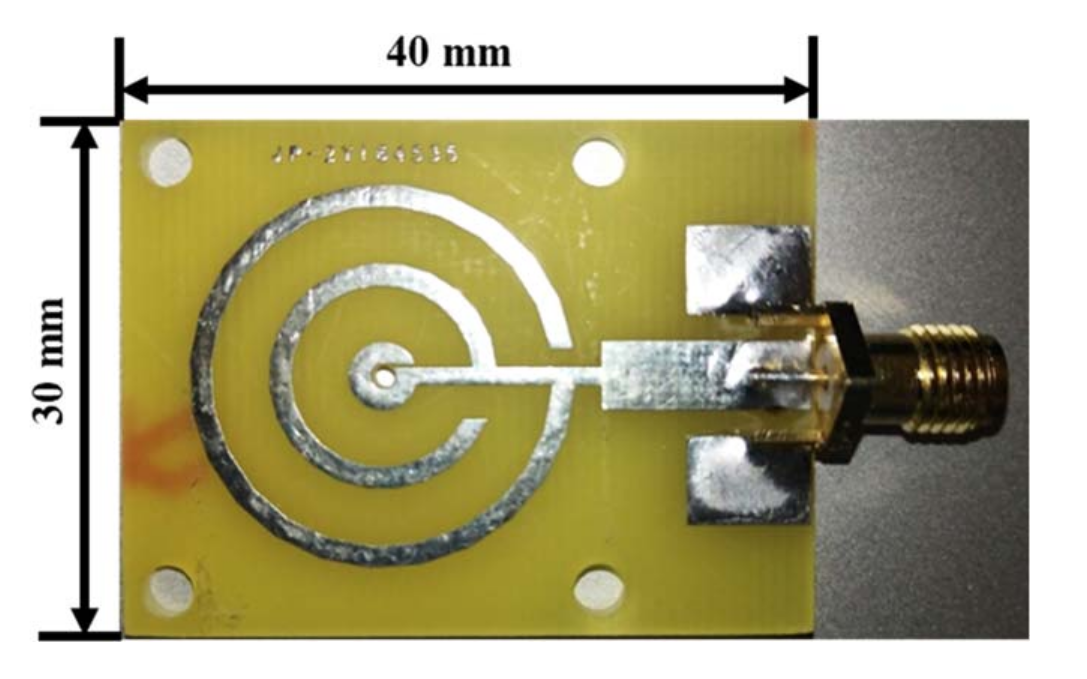
\includegraphics[angle=0,origin=c,width = .8\linewidth]{Section_ODMR_Antenna/Figures/RealAntenna.png}
    \caption{An image of the real antenna used in the reference article. Here \textbf{the thickness of
    the central line, and its length} are not given. The thickness and the length of the central line
	(up to the outer edge of the largest circle) are estimated to be 1.12mm, 1.57mm respectively.}
    \label{fig:RealAntenna}
\end{figure}

Upon estimating the missing dimensions, antenna can be replicated in AutoCAD. It is important
to note that the line thicknesses in the drawing has to be zero (0). Also all the line segments,
arcs, etc. have to be connected so that the final drawing has to have only polylines for disconnected
objects. You can test the polyline behavior by hovering the over lines in the drawing. Once the 
mouse is hovered AutoCAD generates a shade throughout polylines, Figure\ref{fig:ShadedUnshaded}.

\begin{figure}[H]
	\centering
	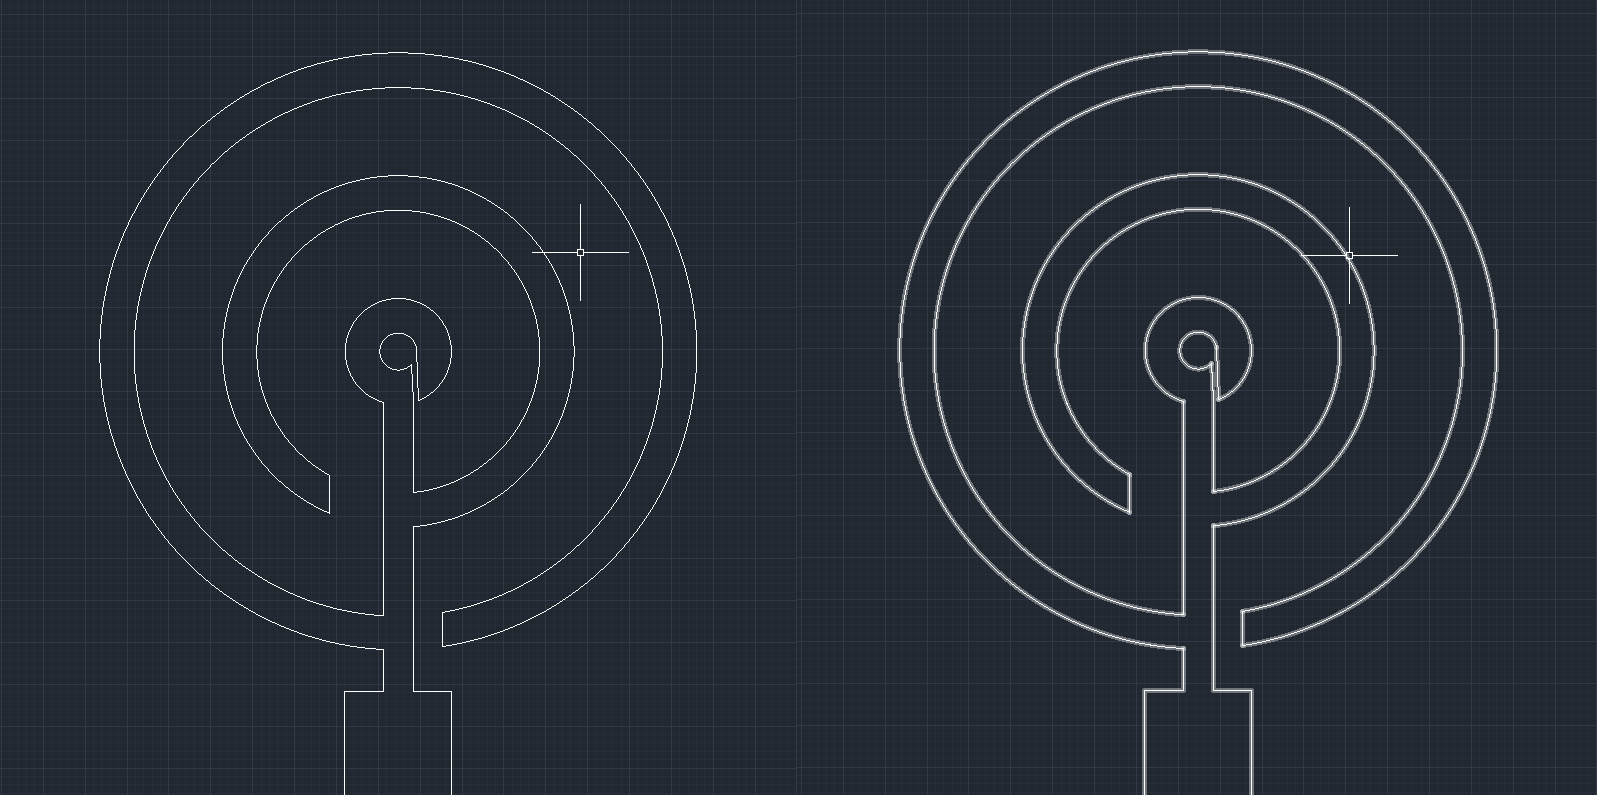
\includegraphics[angle=0,origin=c,width = .8\linewidth]{Section_ODMR_Antenna/Figures/ShadedUnshaded.png}
	\caption{A screenshot from AutoCAD showing the finalized antenna design (\textbf{left}), and
		the shade on polyline when the mouse/cursor is hovered on a line (\textbf{right}).}
	\label{fig:ShadedUnshaded}
\end{figure}

It is important to note that AutoCAD's printing mechanism is a bit complicated. It does not
simply print the drawing in 1:1 scale, neither I recognizes the which paper size is suitable
for the design. Specific to the "Student Version", it also creates watermarks near the side edges
of the print area. These are all required to be handled manually. The conversion of design to .pdf 
format needs to be done in following steps;

\begin{enumerate}
	
	\item Click on the "Print" button, Figure\ref{fig:PrintButton}. This will open up "Plot - Model" window for you,
	Figure\ref{fig:PlotModelWindow}.

	\begin{figure}[H]
		\centering
		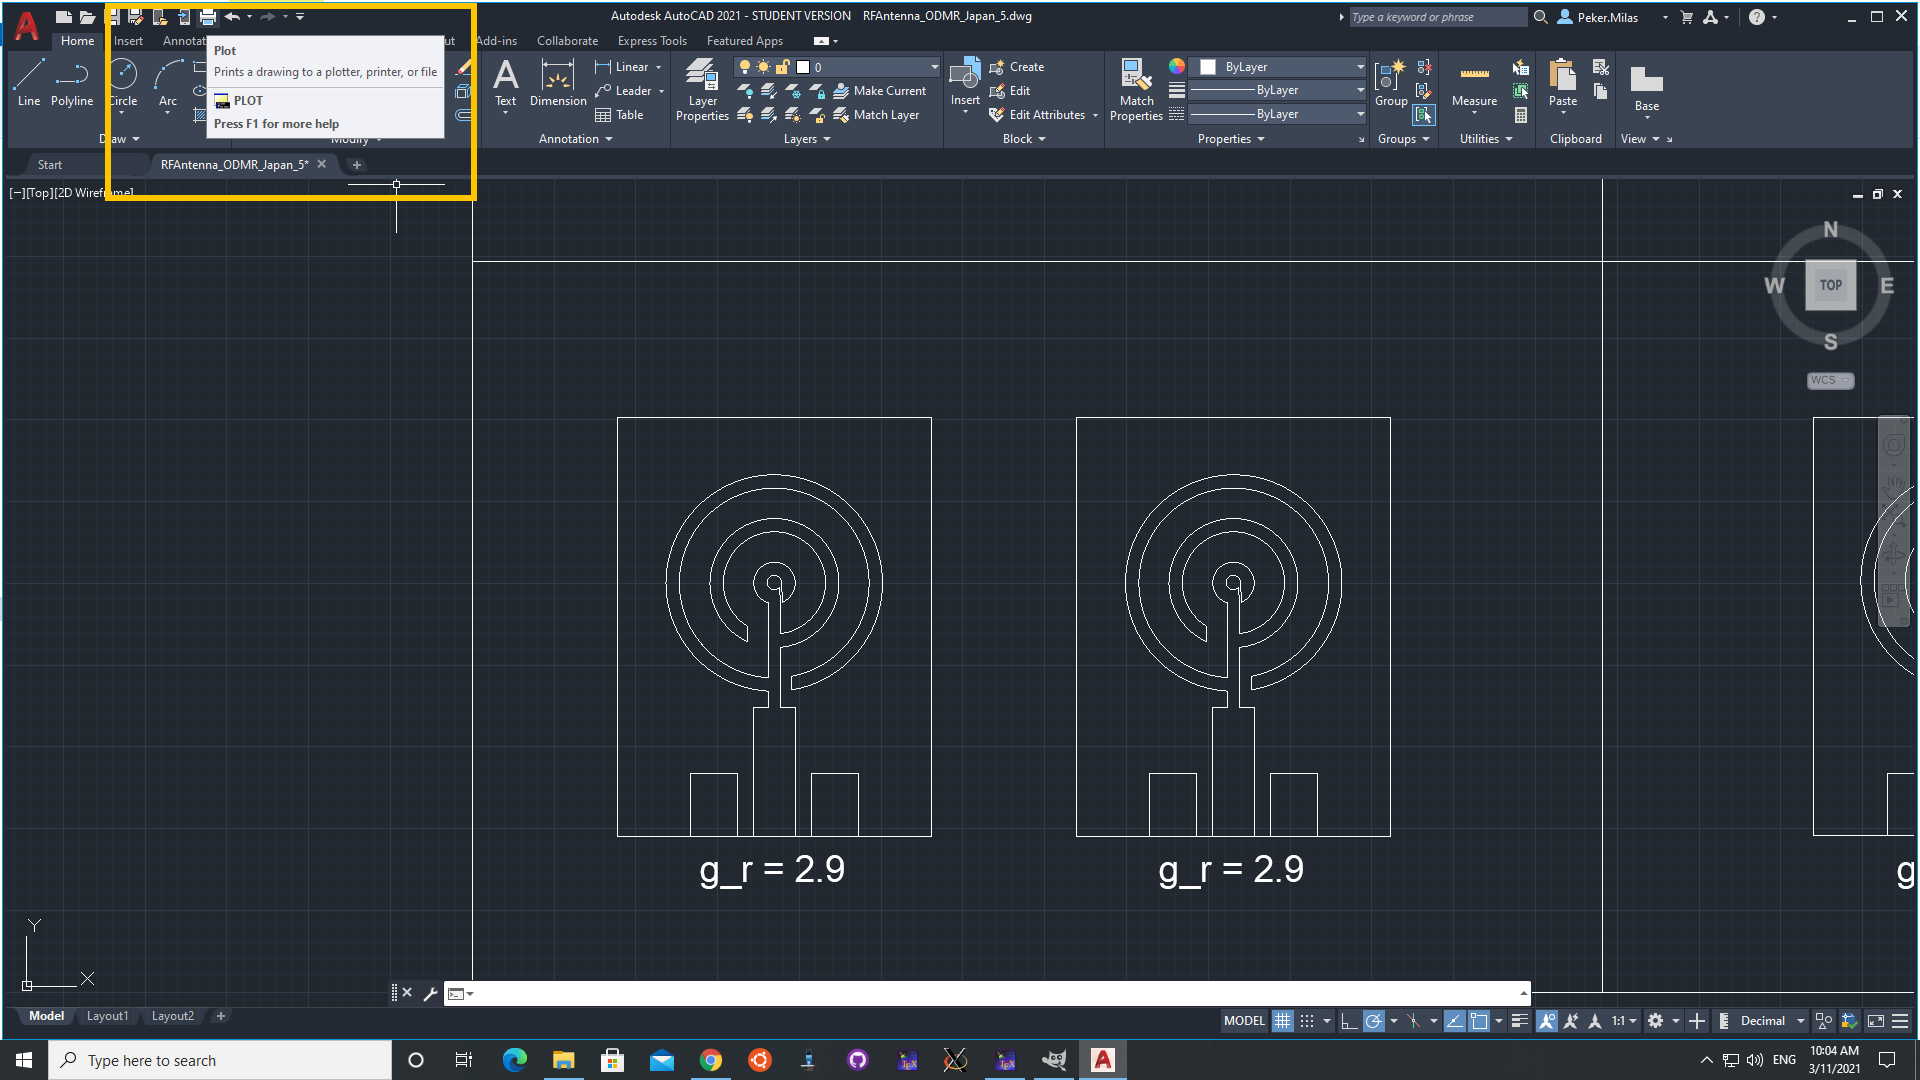
\includegraphics[angle=0,origin=c,width = .8\linewidth]{Section_ODMR_Antenna/Figures/PrintButton.png}
		\caption{"Print" button on AutoCAD top menu.}
		\label{fig:PrintButton}
	\end{figure}
	
	\begin{figure}[H]
		\centering
		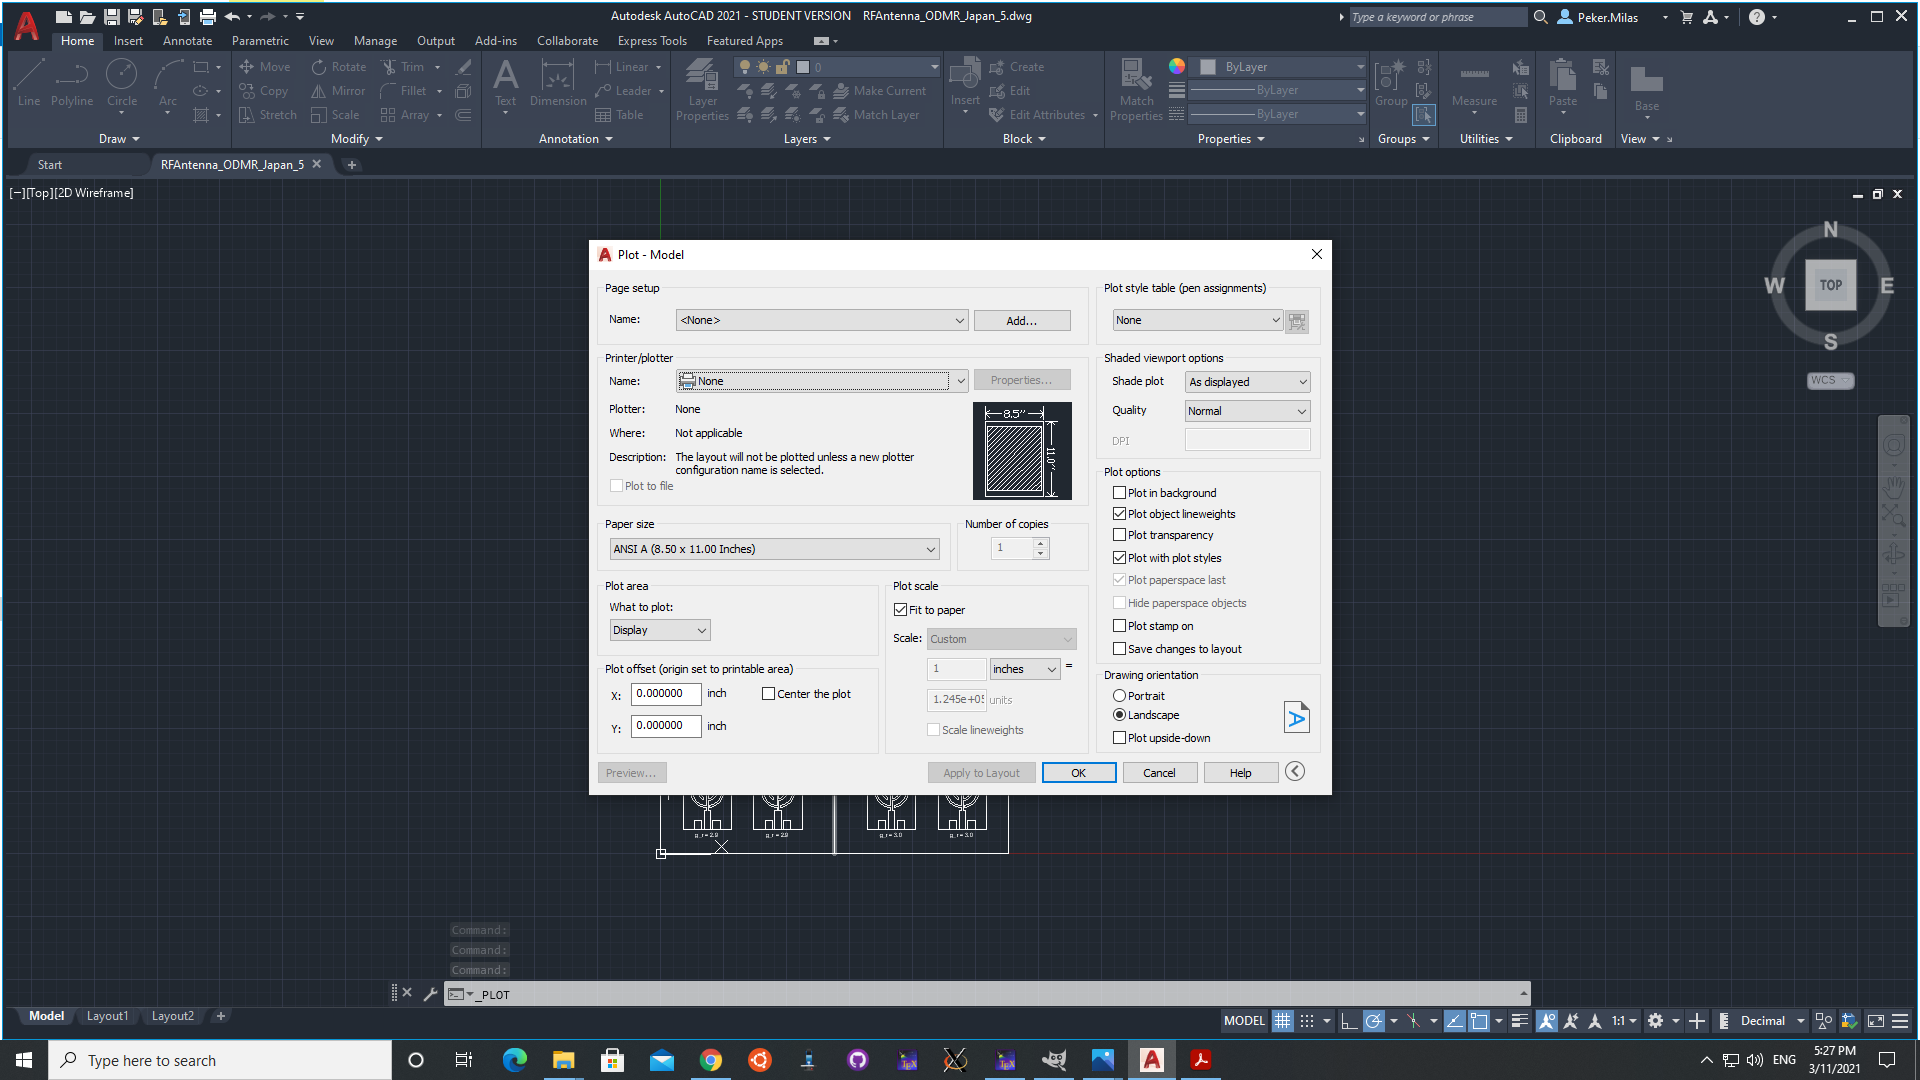
\includegraphics[angle=0,origin=c,width = .8\linewidth]{Section_ODMR_Antenna/Figures/PlotModelWindow.png}
		\caption{"Plot - Model" window in AutoCAD.}
		\label{fig:PlotModelWindow}
	\end{figure}

	\item In "Plot - Model" window, select proper "Drawing Orientation" (here \underline{Portrait}),
	Figure\ref{fig:PrintOpenScreen}.

	\begin{figure}[H]
		\centering
		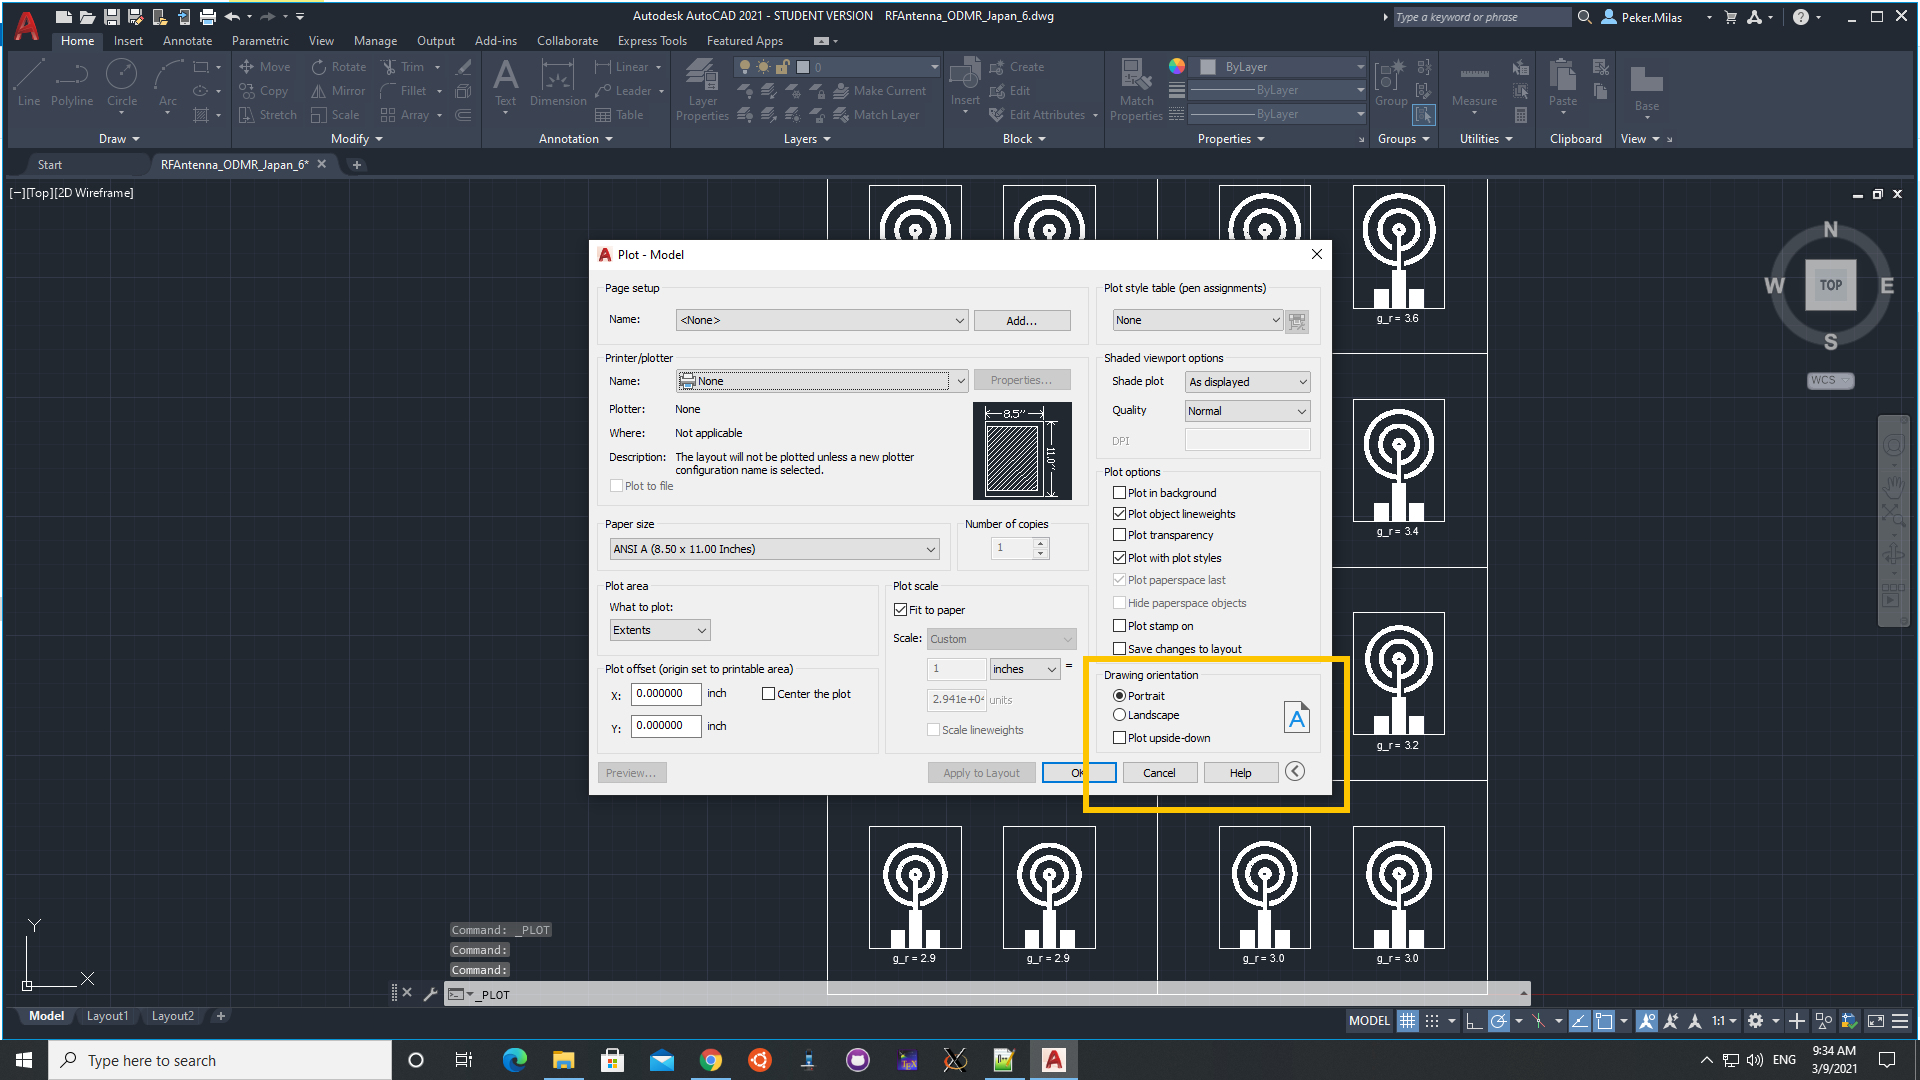
\includegraphics[angle=0,origin=c,width = .8\linewidth]{Section_ODMR_Antenna/Figures/PrintOpenScreen.png}
		\caption{Drawing Orientation section in "Plot - Model" window in AutoCAD.}
		\label{fig:PrintOpenScreen}
	\end{figure}

	\item In "Plot - Model" window, under Printer/plotter section, select AutoCAD PDF (High Quality Print).pc3, 
	Figure\ref{fig:ChoosePlotter1}.

	\begin{figure}[H]
		\centering
		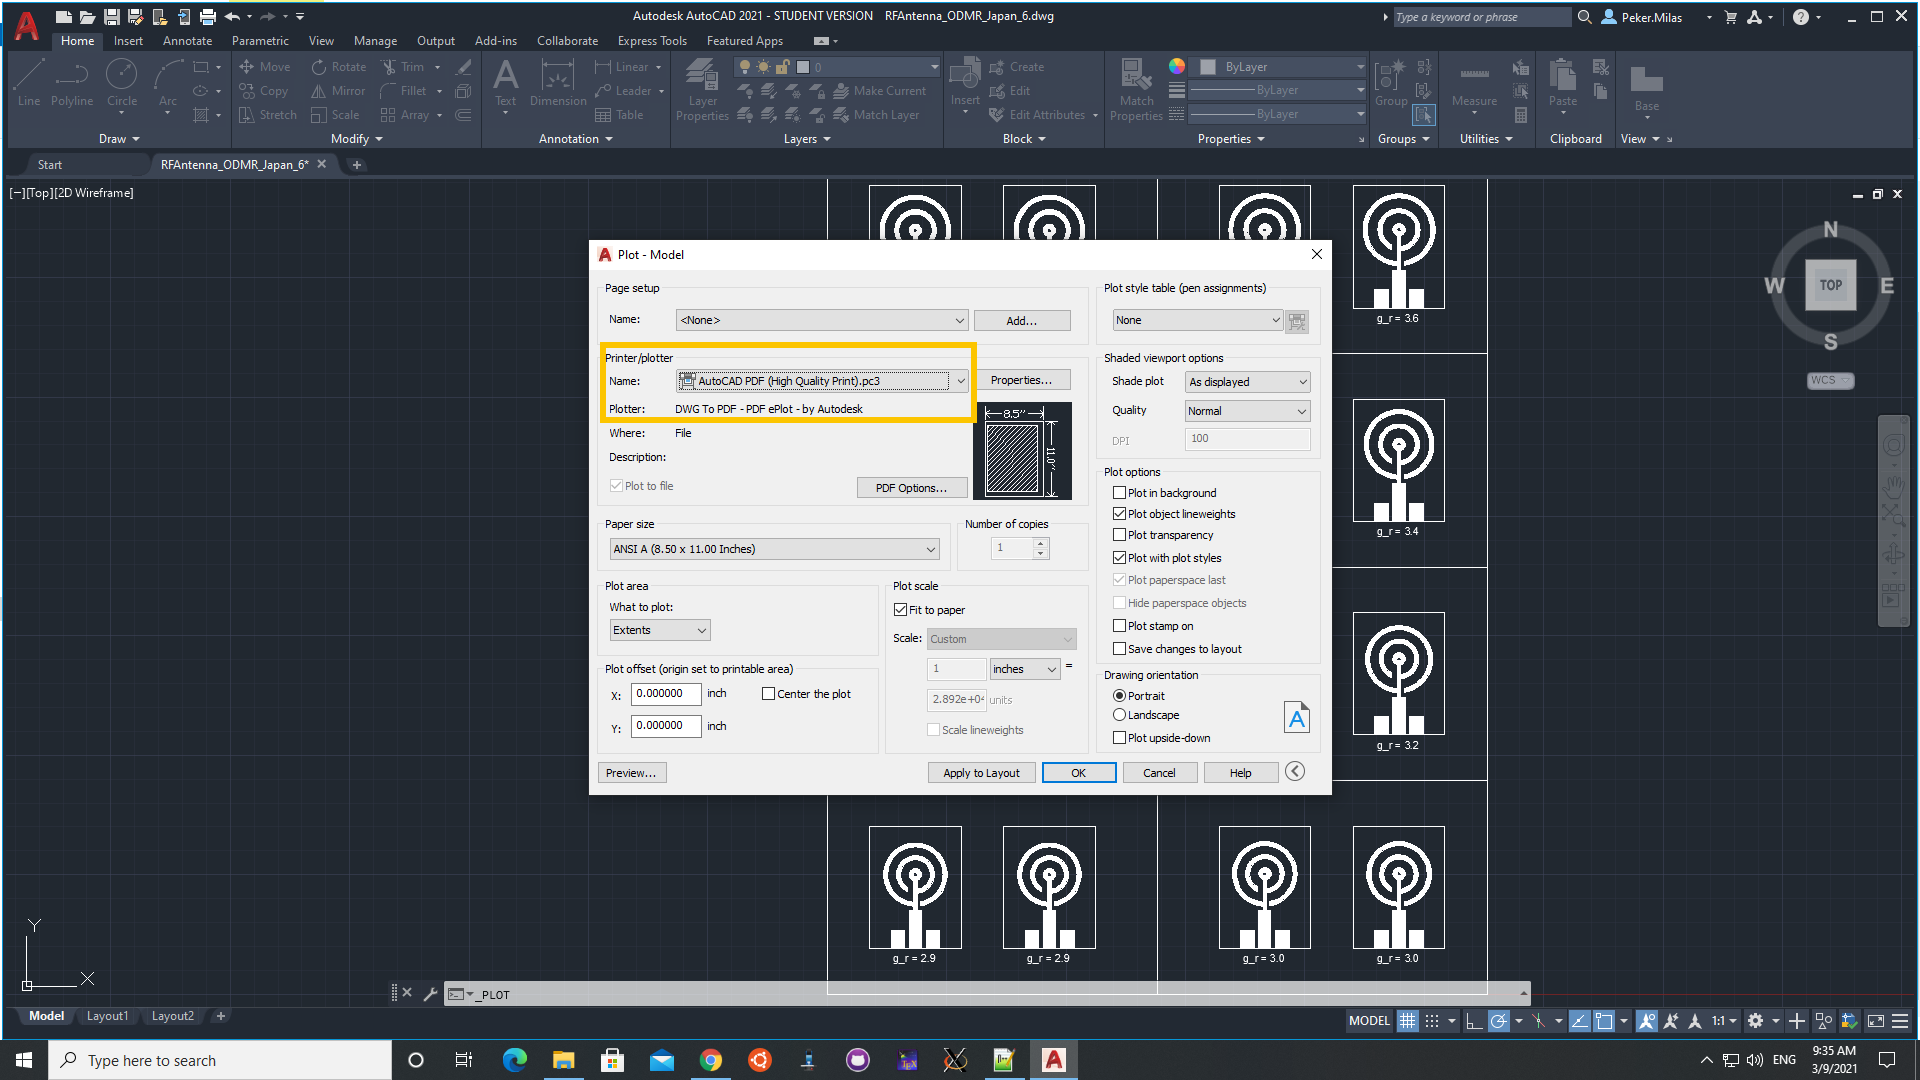
\includegraphics[angle=0,origin=c,width = .8\linewidth]{Section_ODMR_Antenna/Figures/ChoosePlotter1.png}
		\caption{Selection of AutoCAD PDF (High Quality Print).pc3 in Printer/plotter section of "Plot - Model" 
			window in AutoCAD.}
		\label{fig:ChoosePlotter1}
	\end{figure}

	\item In "Plot - Model" window, under Printer/plotter section, select click on PDF Options button, 
	Figure\ref{fig:CustomizePlotter}. This will open up "PDF Options" window, Figure\ref{fig:PDFOptionsWindow}.

	\begin{figure}[H]
		\centering
		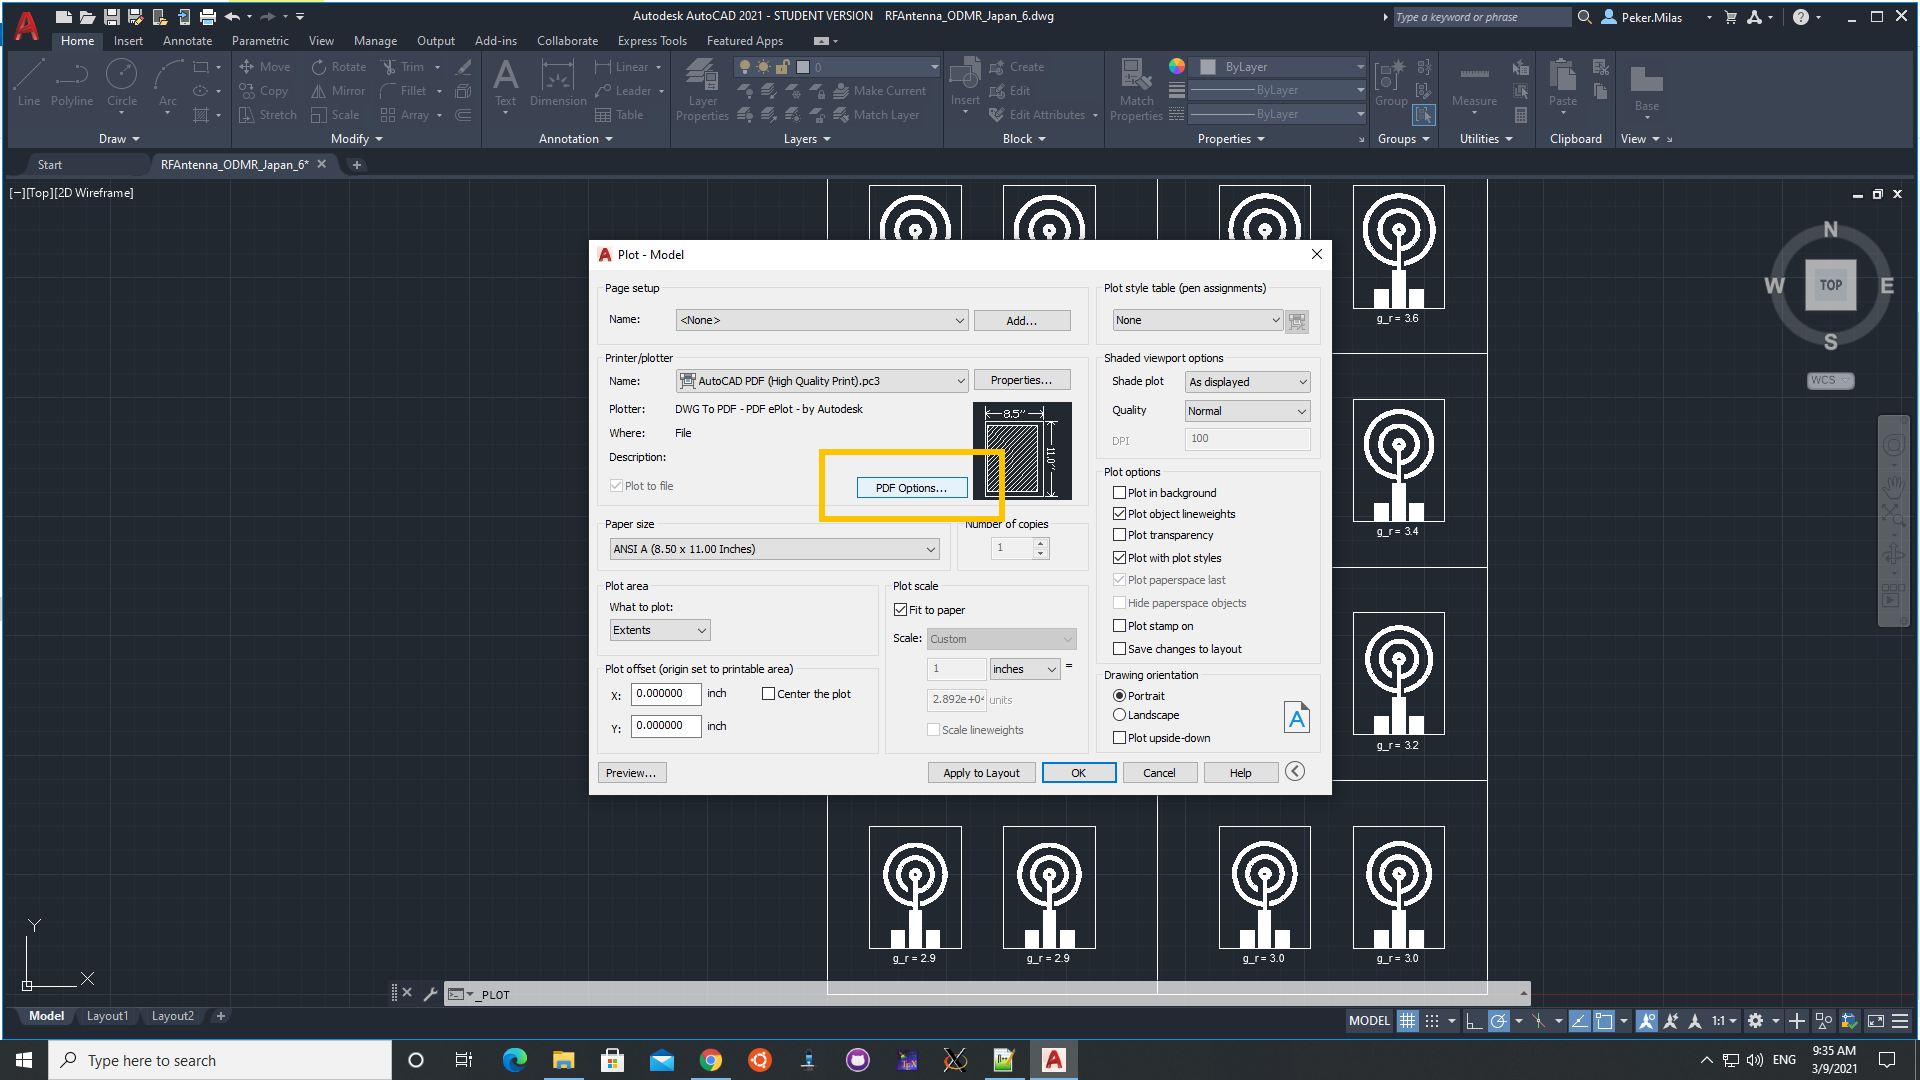
\includegraphics[angle=0,origin=c,width = .8\linewidth]{Section_ODMR_Antenna/Figures/CustomizePlotter.png}
		\caption{PDF Options in Printer/plotter section of "Plot - Model" window in AutoCAD.}
		\label{fig:CustomizePlotter}
	\end{figure}
	
	\begin{figure}[H]
		\centering
		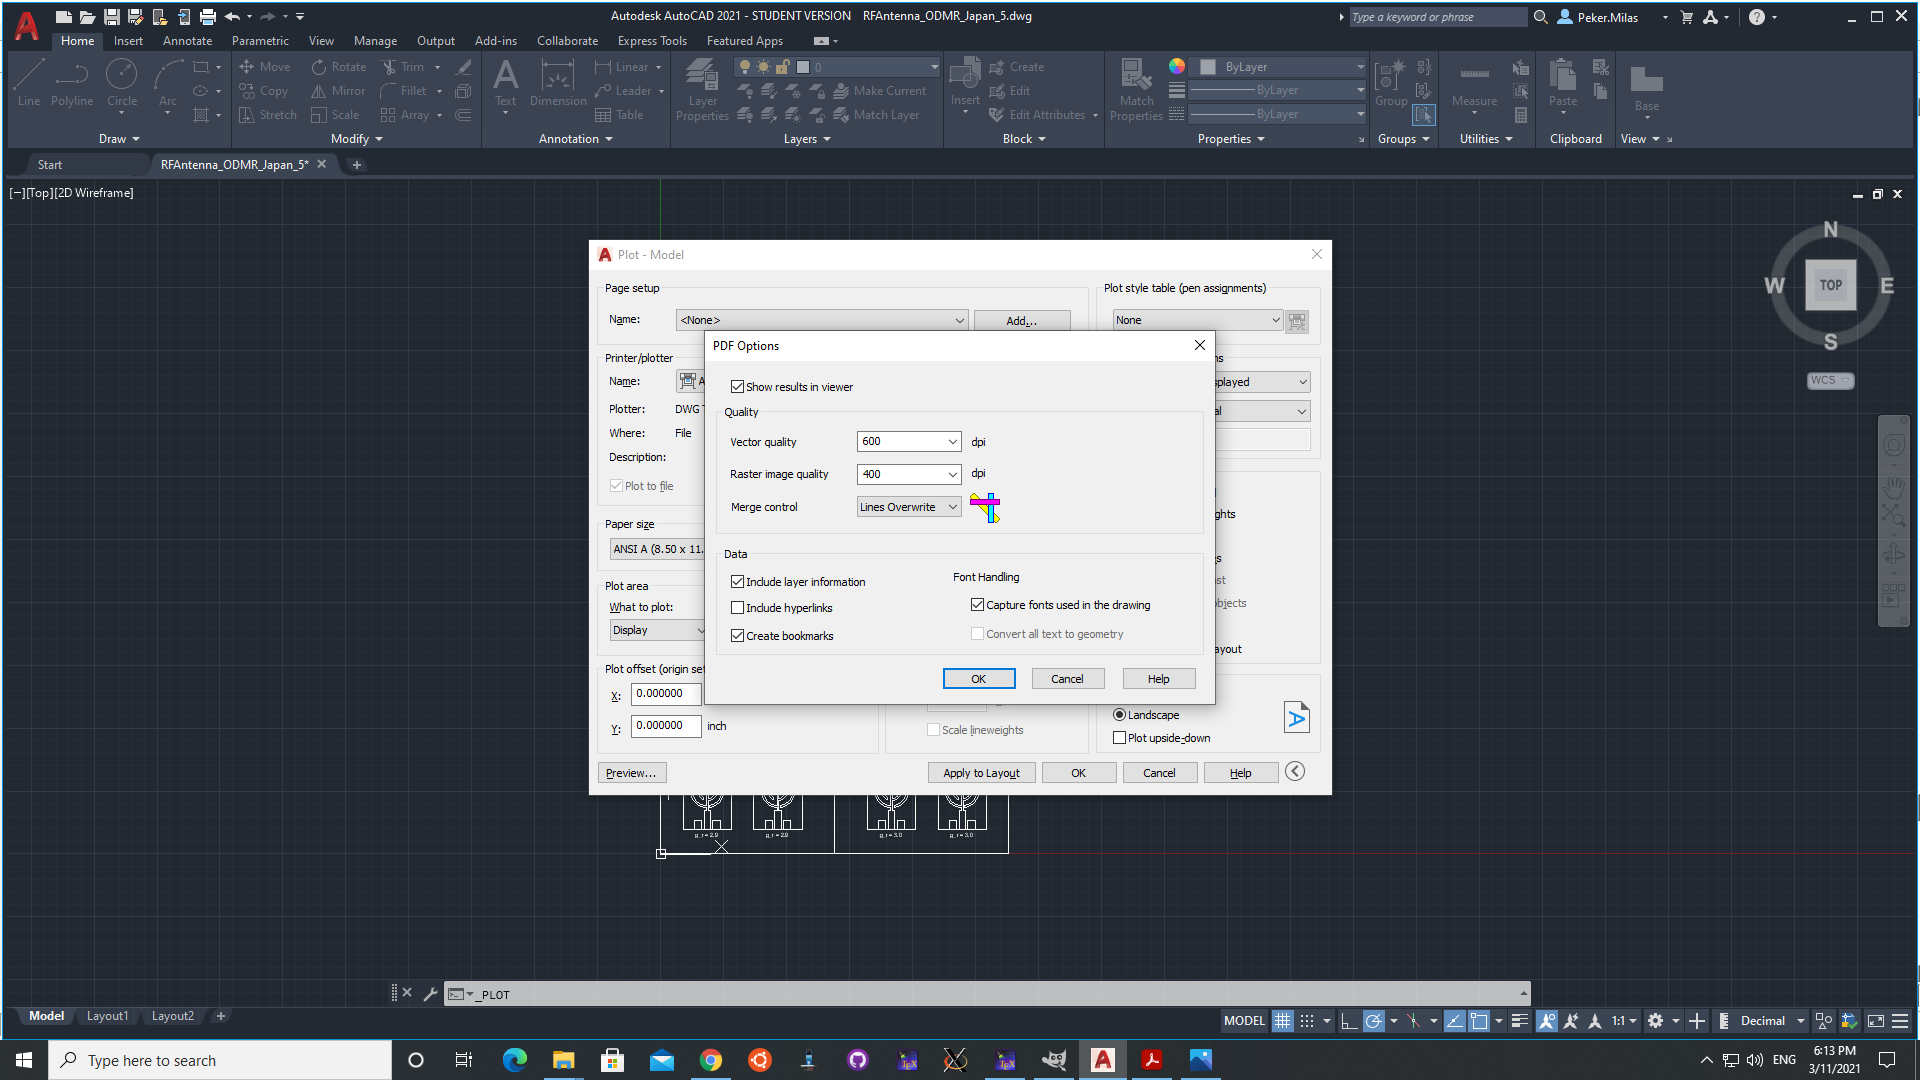
\includegraphics[angle=0,origin=c,width = .8\linewidth]{Section_ODMR_Antenna/Figures/PDFOptionsWindow.png}
		\caption{"PDF Options" window in AutoCAD.}
		\label{fig:PDFOptionsWindow}
	\end{figure}

	\item In "PDF Options" window, under "Quality" section, change both "Vector quality" and "Raster image quality"
	to maximum (4800 dpi), Figure\ref{fig:PDFOptionsWindow1}. Then click on "OK" to close the window.

	\begin{figure}[H]
		\centering
		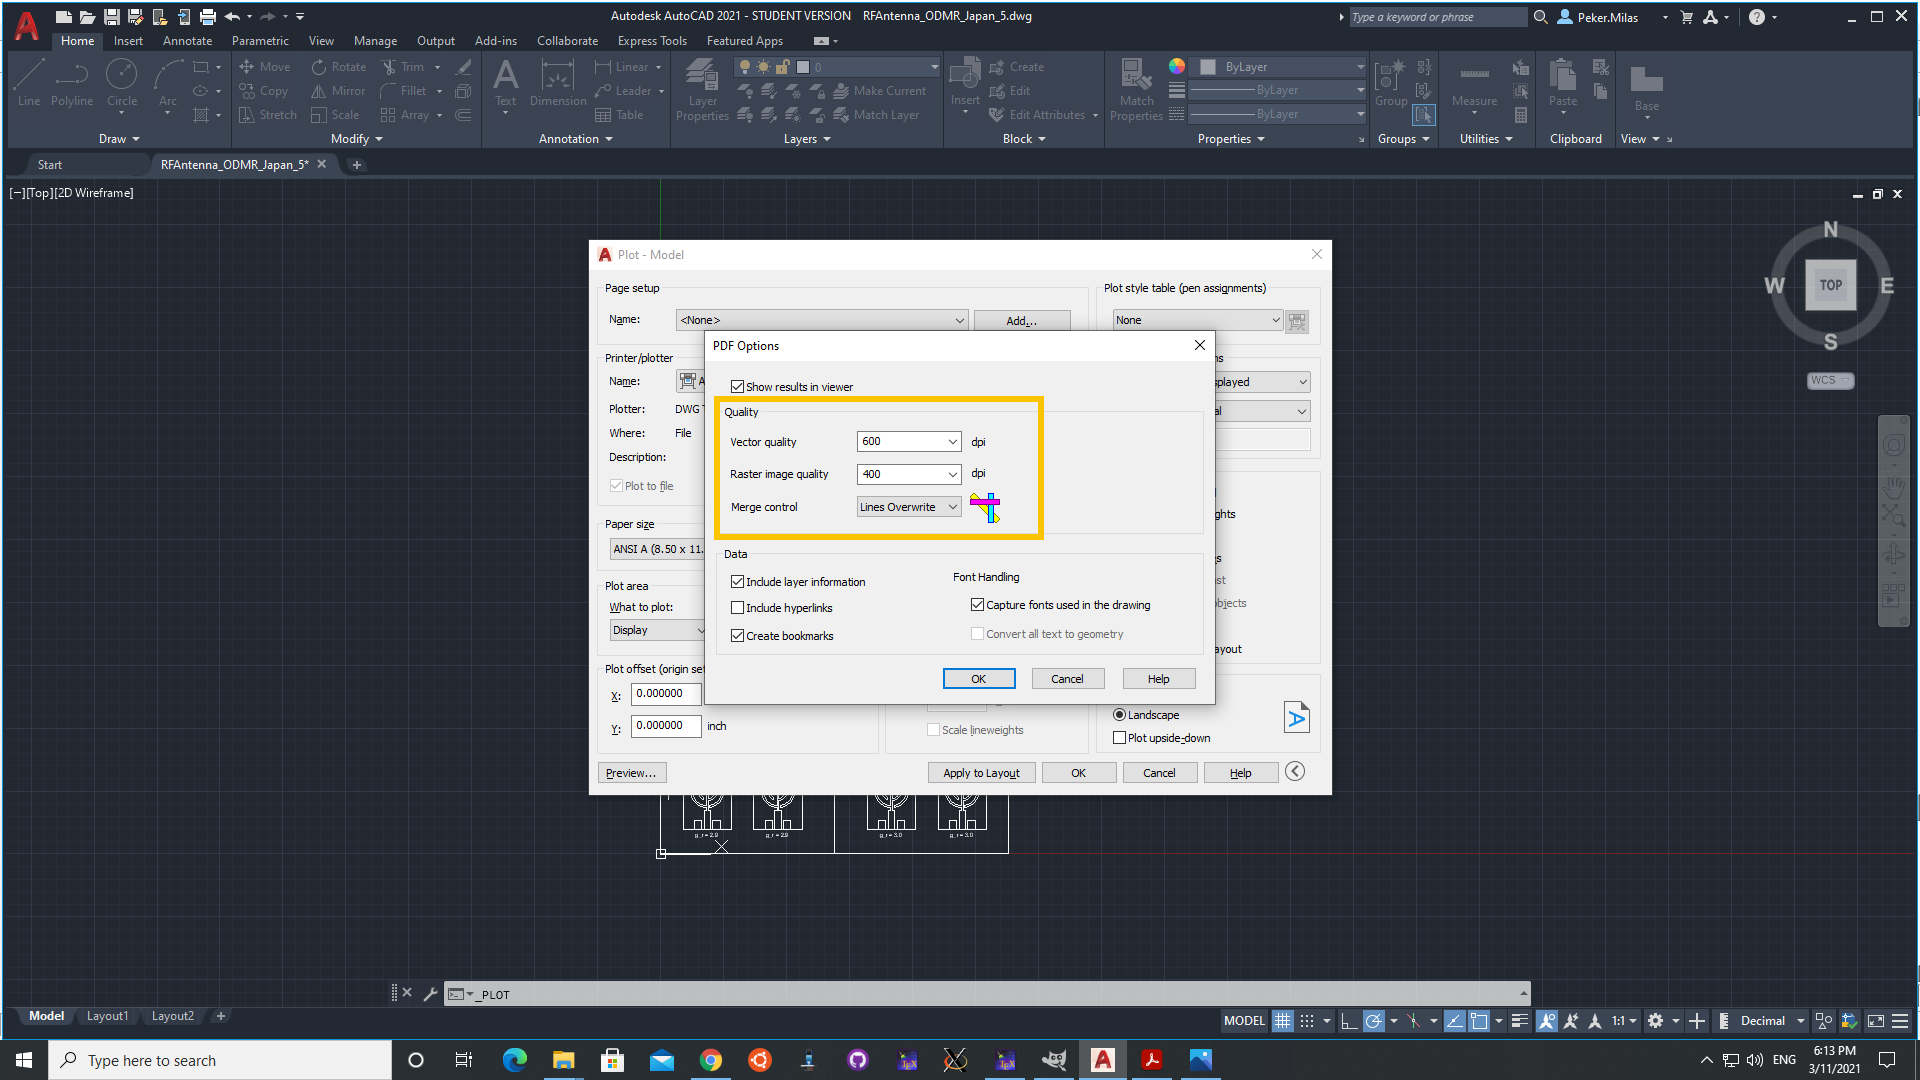
\includegraphics[angle=0,origin=c,width = .8\linewidth]{Section_ODMR_Antenna/Figures/PDFOptionsWindow1.png}
		\caption{"PDF Options" window in AutoCAD.}
		\label{fig:PDFOptionsWindow1}
	\end{figure}

	\item In "Plot - Model" window, under Printer/plotter section, click on the "Properties" button. This will open 
	up "Plotter Configuration Editor", Figure\ref{fig:CustomizePaperSize}.
	
	\begin{figure}[H]
		\centering
		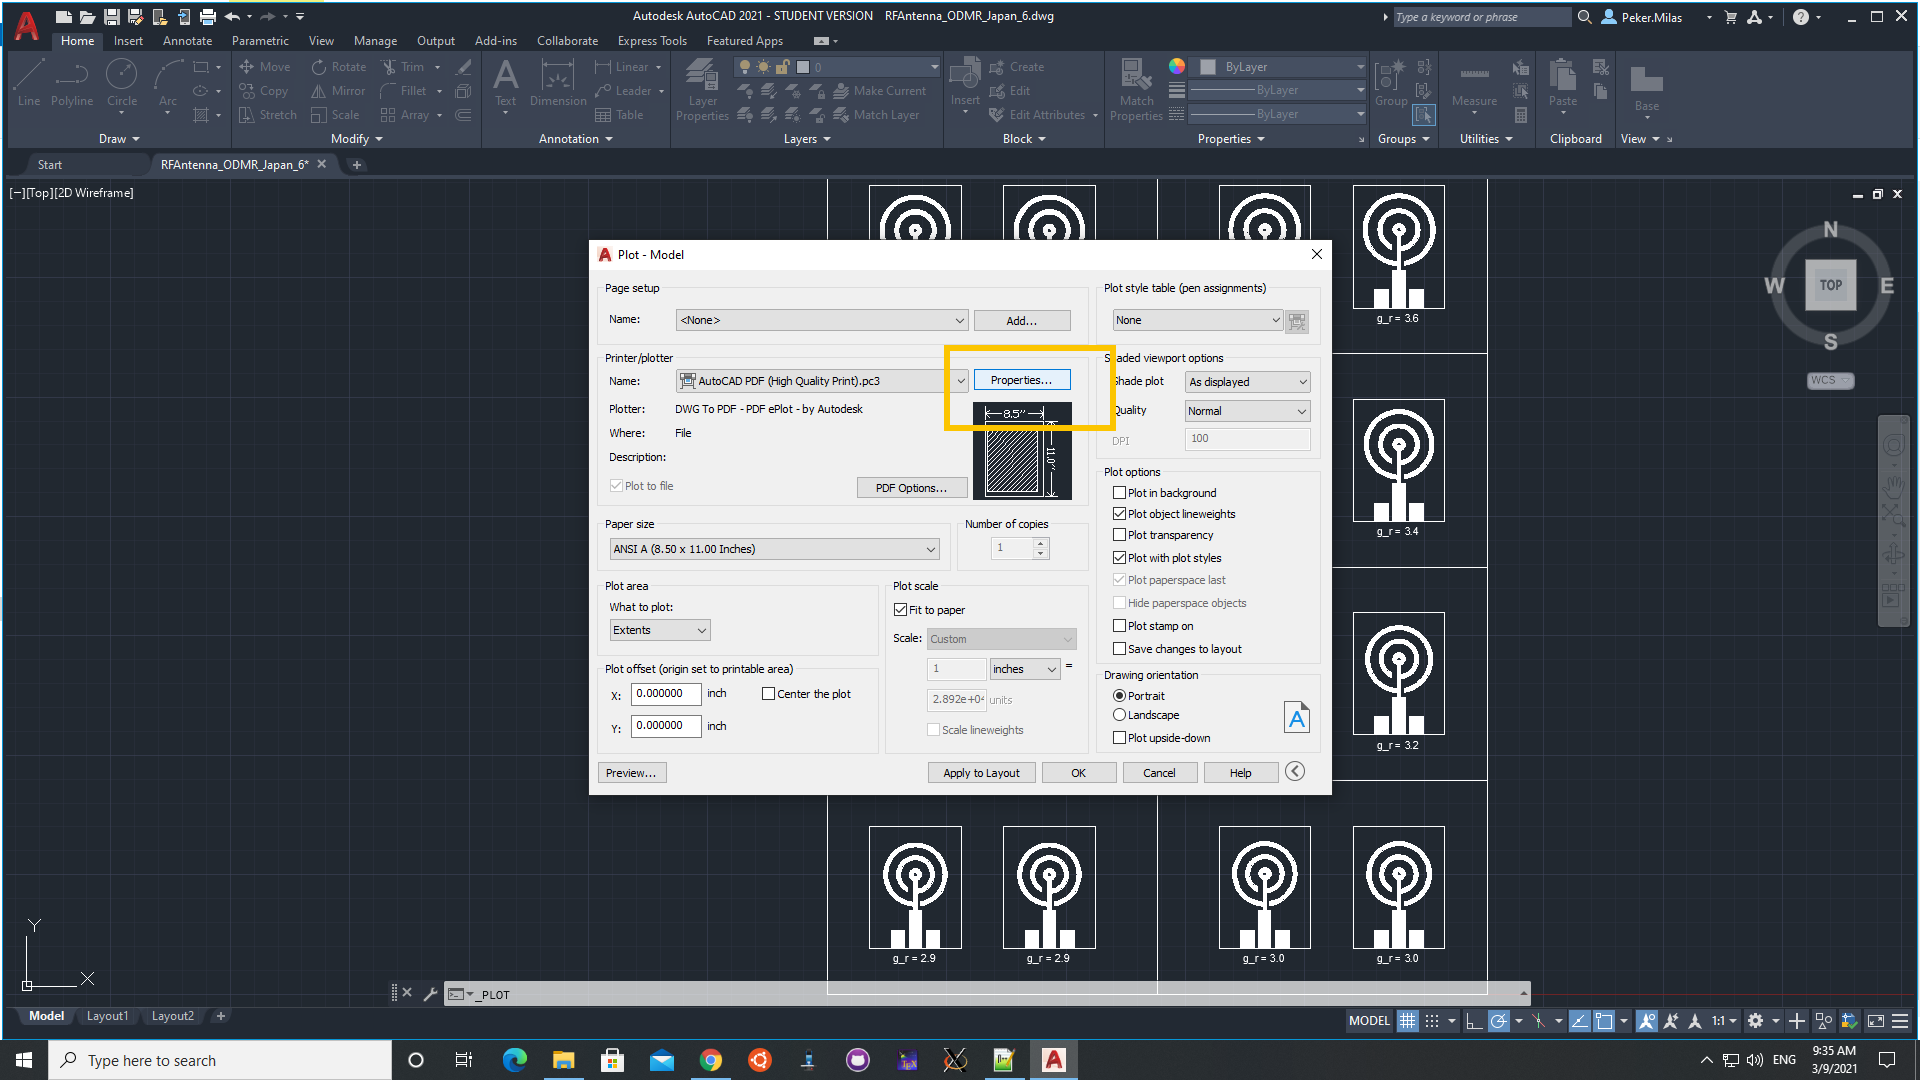
\includegraphics[angle=0,origin=c,width = .8\linewidth]{Section_ODMR_Antenna/Figures/CustomizePaperSize.png}
		\caption{"Properties" button in Printer/plotter section of "Plot - Model" window in AutoCAD.}
		\label{fig:CustomizePaperSize}
	\end{figure}
	
	\item In "Plotter Configuration Editor" window, select "Modify Standard Paper Sizes", 
	Figure\ref{fig:ChoosePaperType1} and select proper paper type (here ANSI A (8.50 x 11.00 Inches)),
	Figure\ref{fig:ChoosePaperType2} in the "Modify Standard Paper Sizes" section.

	\begin{figure}[H]
		\centering
		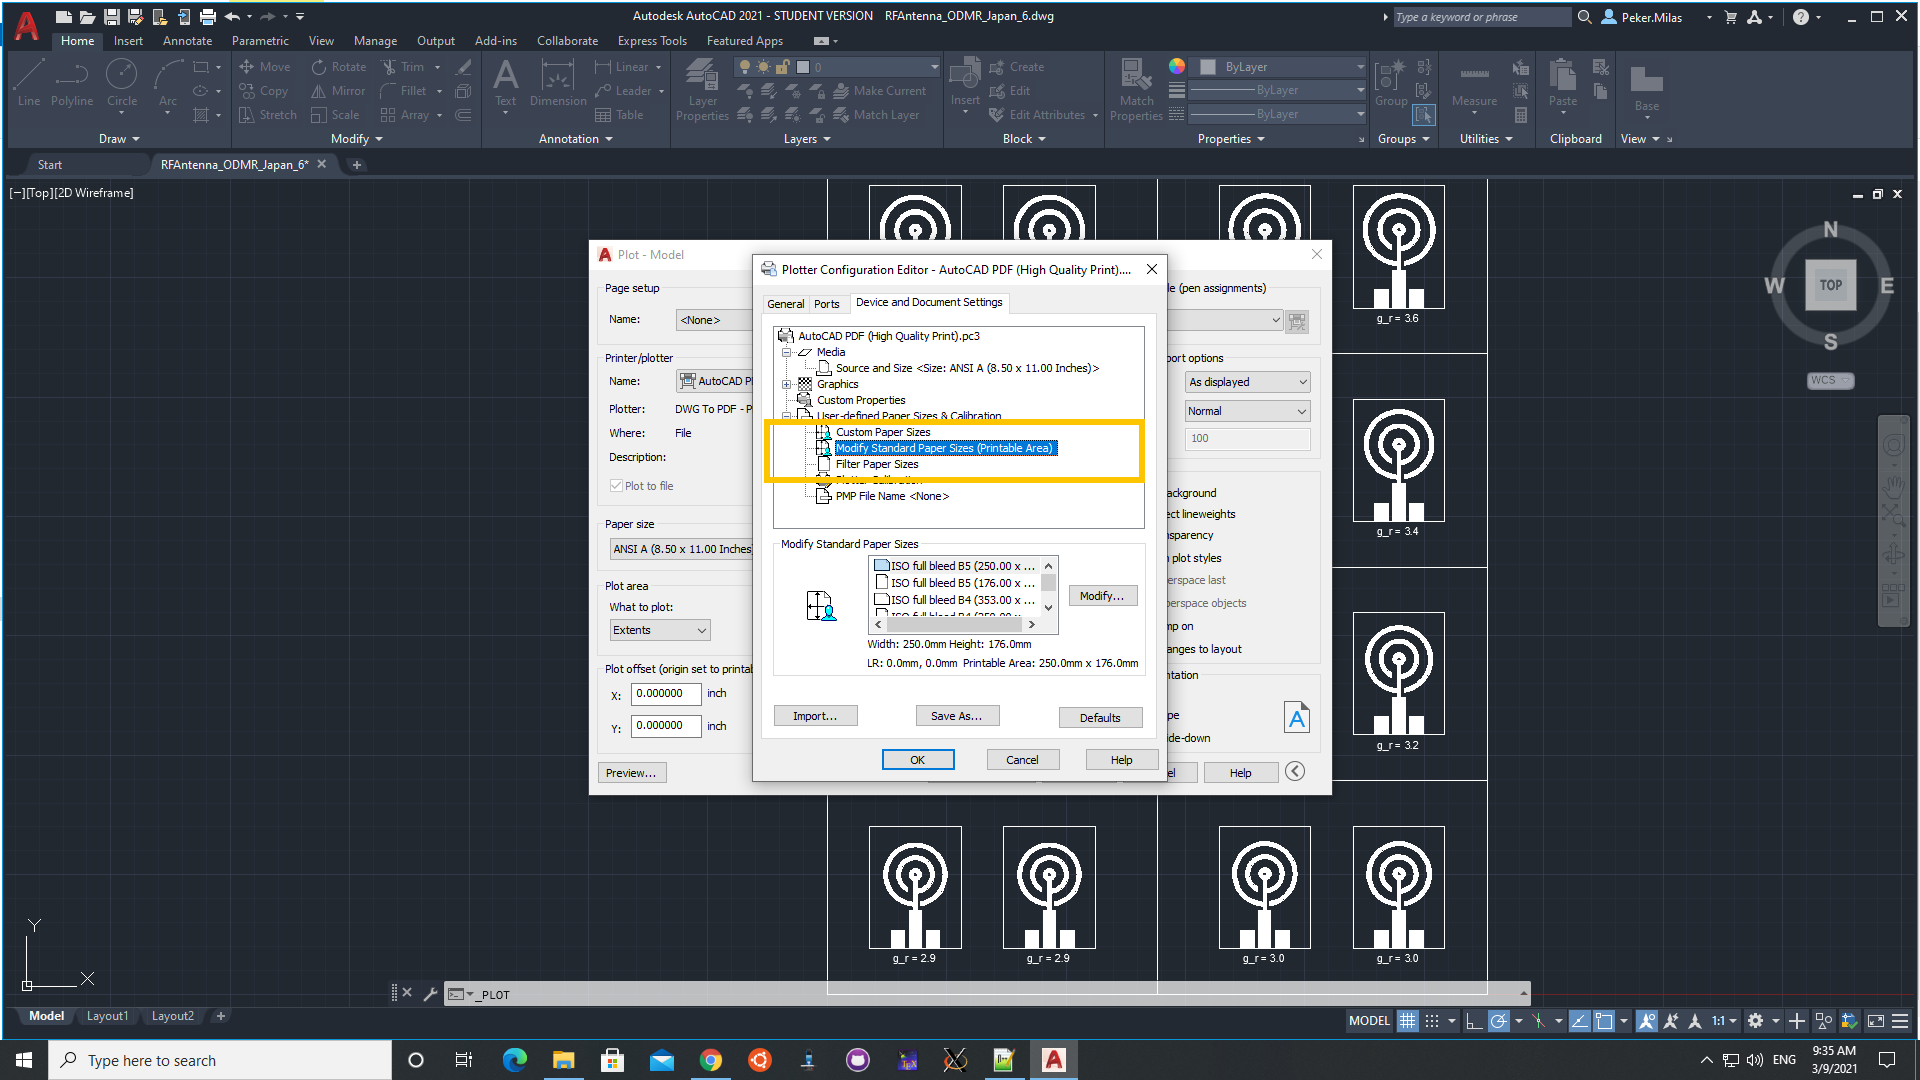
\includegraphics[angle=0,origin=c,width = .8\linewidth]{Section_ODMR_Antenna/Figures/ChoosePaperType1.png}
		\caption{In "Plotter Configuration Editor", selection of "Modify Standard Paper Sizes" in AutoCAD.}
		\label{fig:ChoosePaperType1}
	\end{figure}

	\begin{figure}[H]
		\centering
		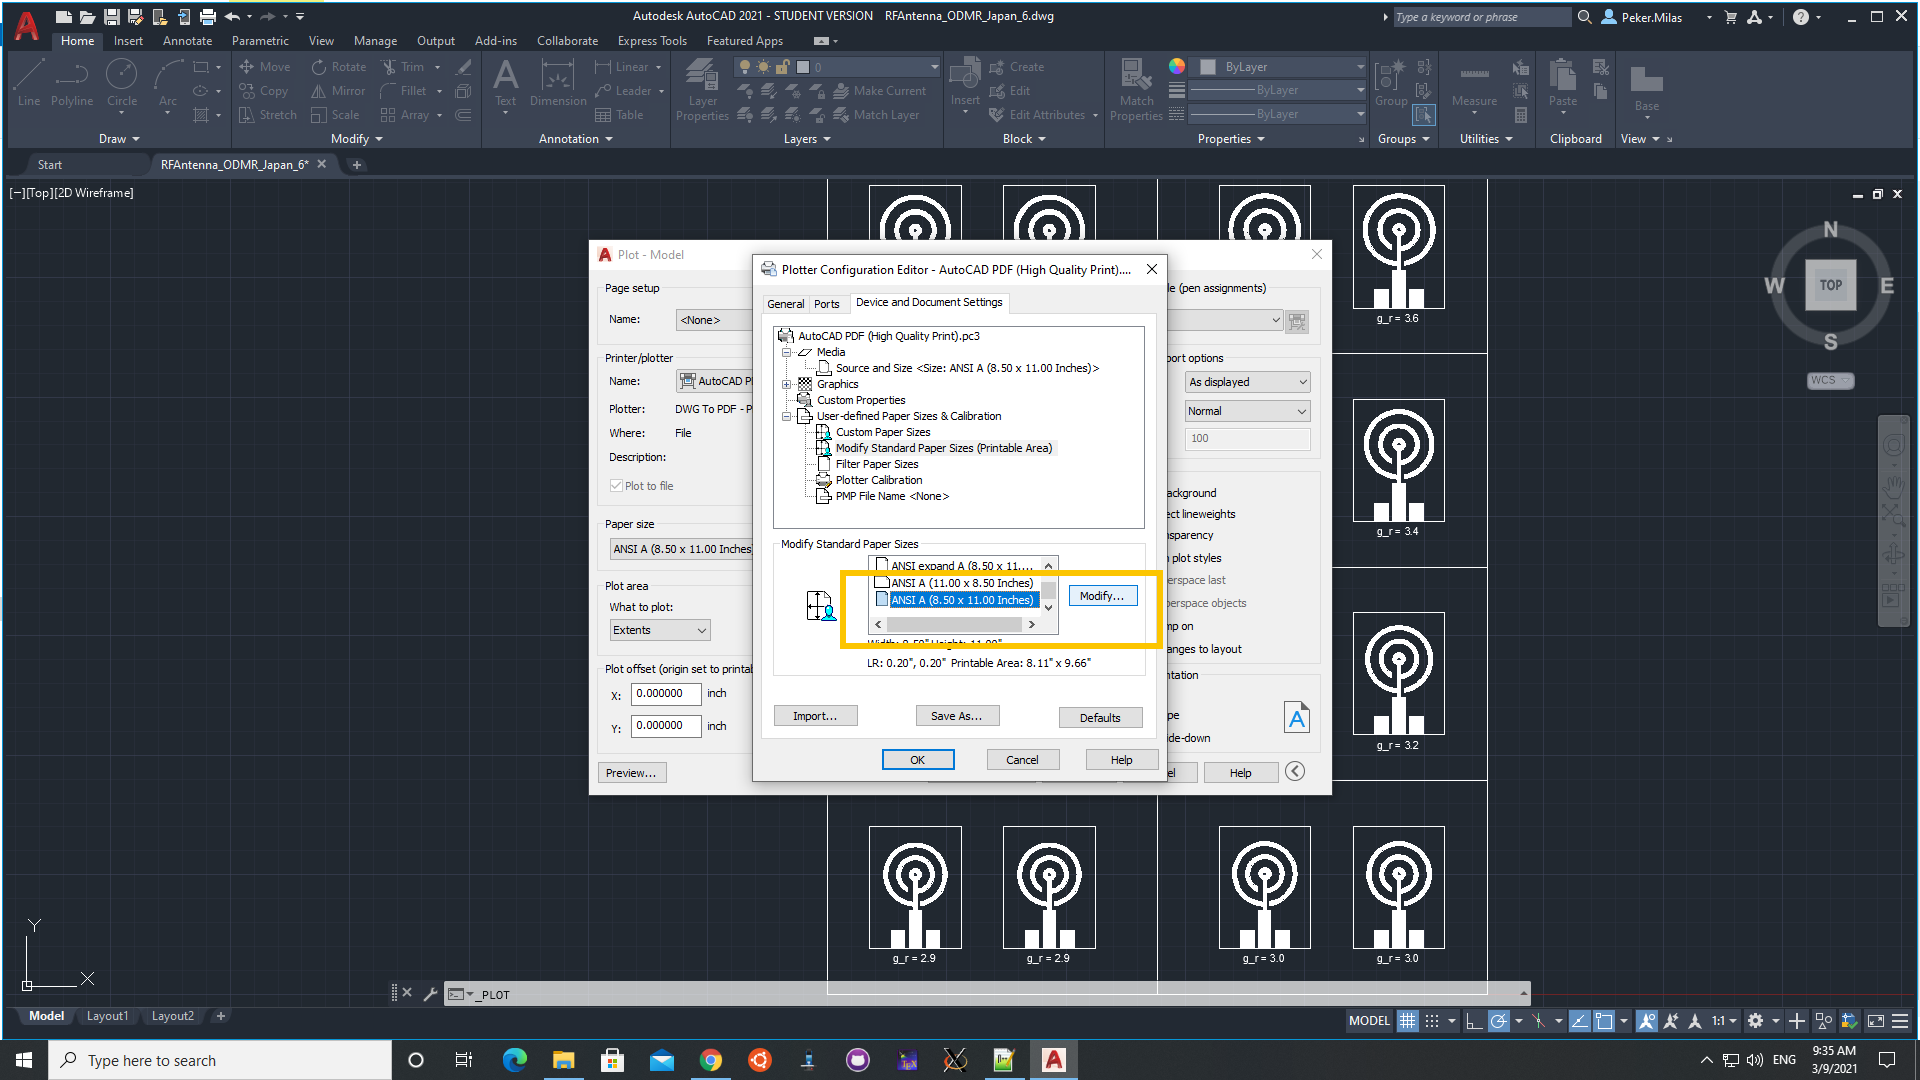
\includegraphics[angle=0,origin=c,width = .8\linewidth]{Section_ODMR_Antenna/Figures/ChoosePaperType2.png}
		\caption{In "Plotter Configuration Editor", paper type selection in AutoCAD.}
		\label{fig:ChoosePaperType2}
	\end{figure}

	\item Click on the "Modify" button in "Modify Standard Paper Sizes" section. This will open up 
	"Custom Paper Size - Printable Area" window for you, Figure\ref{fig:ChangePaperMargins1}.
	
	\begin{figure}[H]
		\centering
		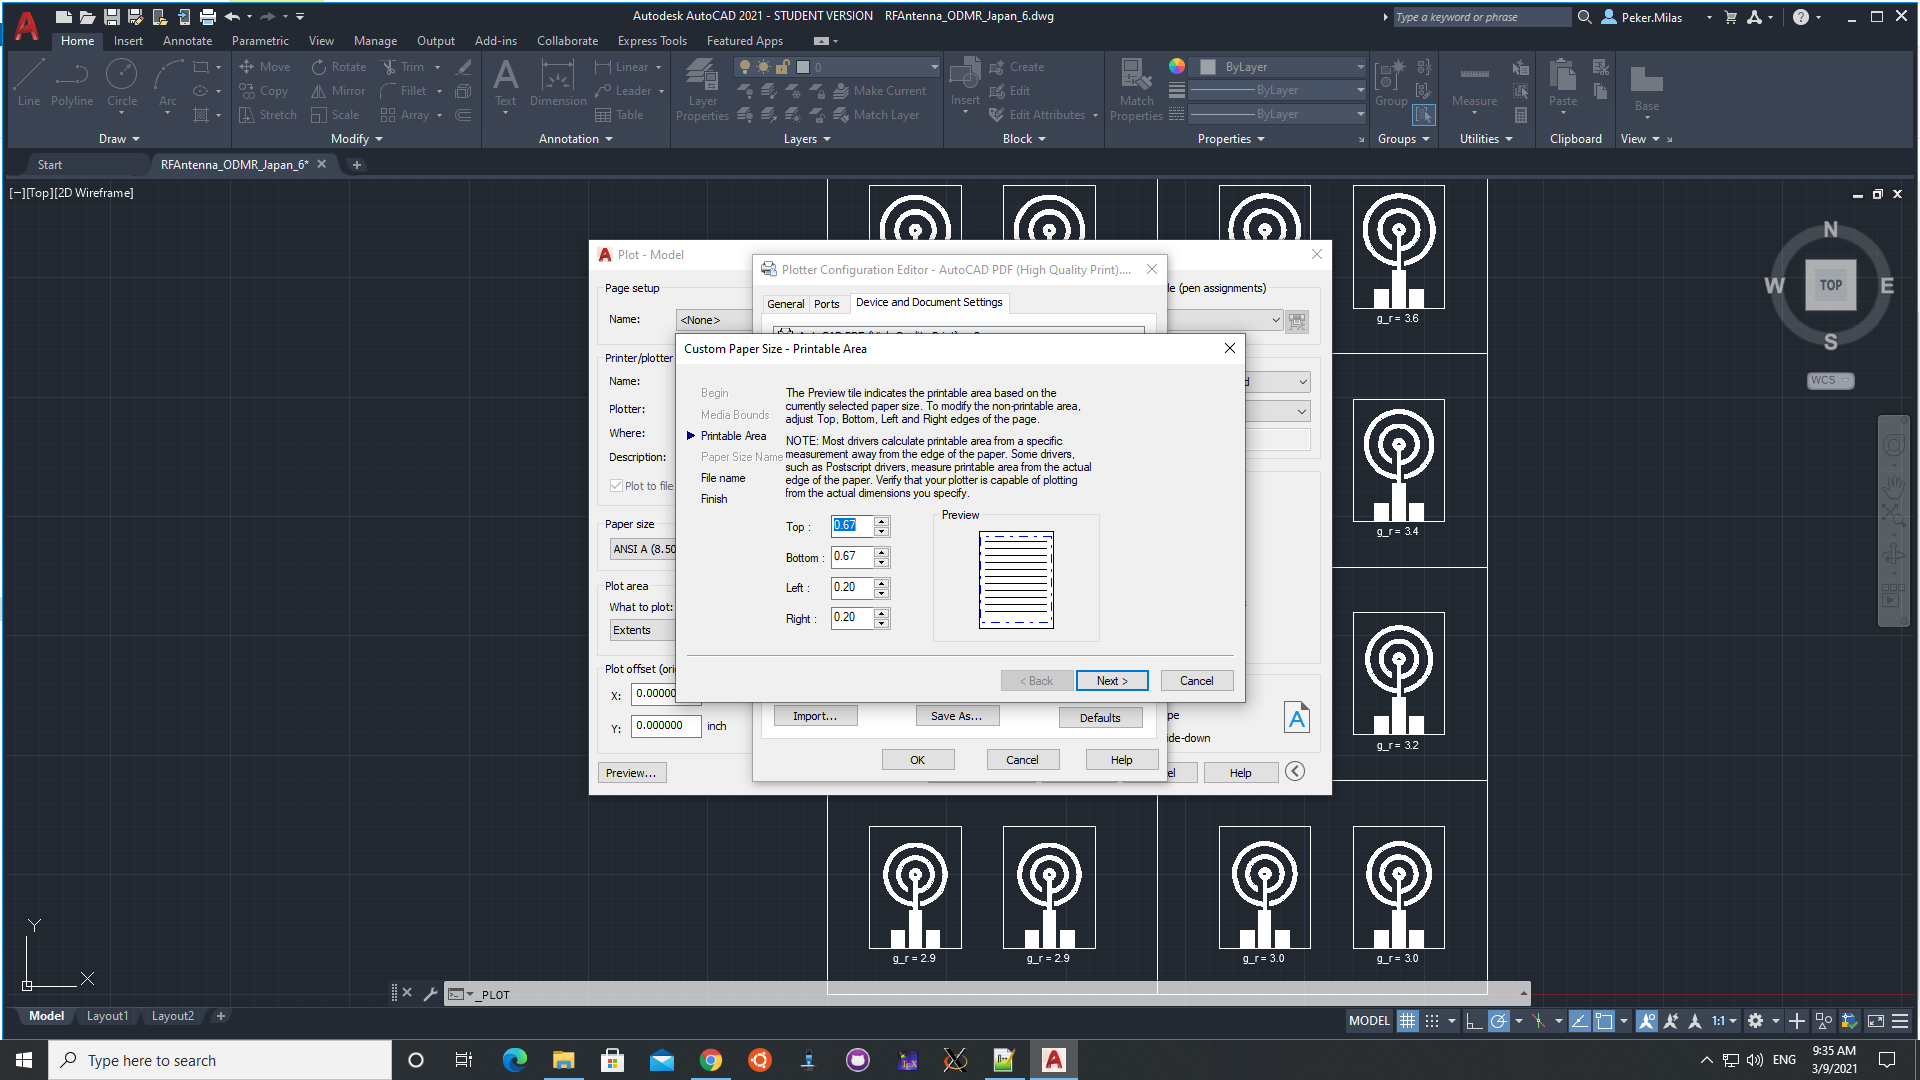
\includegraphics[angle=0,origin=c,width = .8\linewidth]{Section_ODMR_Antenna/Figures/ChangePaperMargins1.png}
		\caption{"Custom Paper Size - Printable Area" window in AutoCAD.}
		\label{fig:ChangePaperMargins1}
	\end{figure}
	
	\item In "Custom Paper Size - Printable Area" window, change the values for Top-Bottom-Right-Left to
	zero (0), Figure\ref{fig:ChangePaperMargins2}.
	
	\begin{figure}[H]
		\centering
		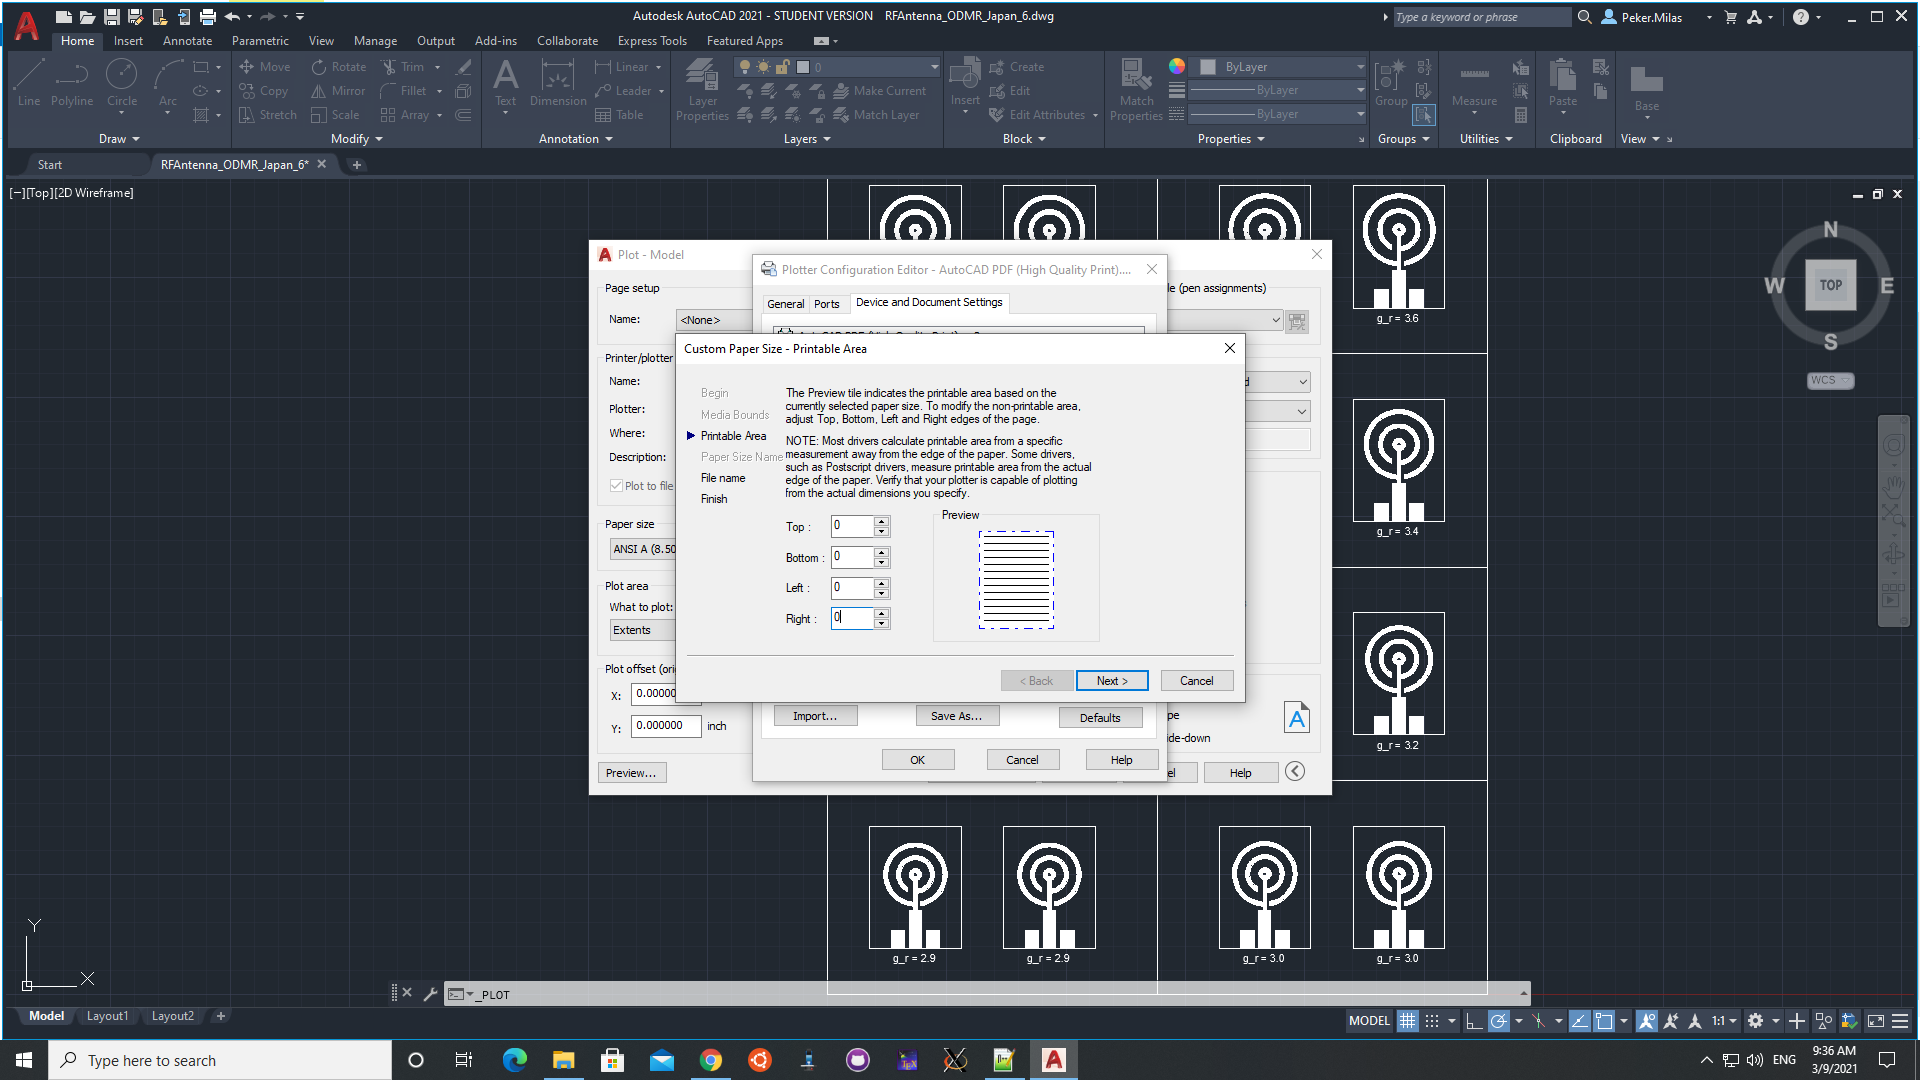
\includegraphics[angle=0,origin=c,width = .8\linewidth]{Section_ODMR_Antenna/Figures/ChangePaperMargins2.png}
		\caption{Setting print margins to zero in "Custom Paper Size - Printable Area" window.}
		\label{fig:ChangePaperMargins2}
	\end{figure}
	
	\item Click on "Next", then "Next", and finally "Finish". This will change the plotter settings and create 
	a new file in AutoCAD/Plotters/PMP files directory, Figure\ref{fig:FolderOfCustomPlotters}. Once conversion to 
	.pdf is done, it is a good practice to delete this file.
	
	\begin{figure}[H]
		\centering
		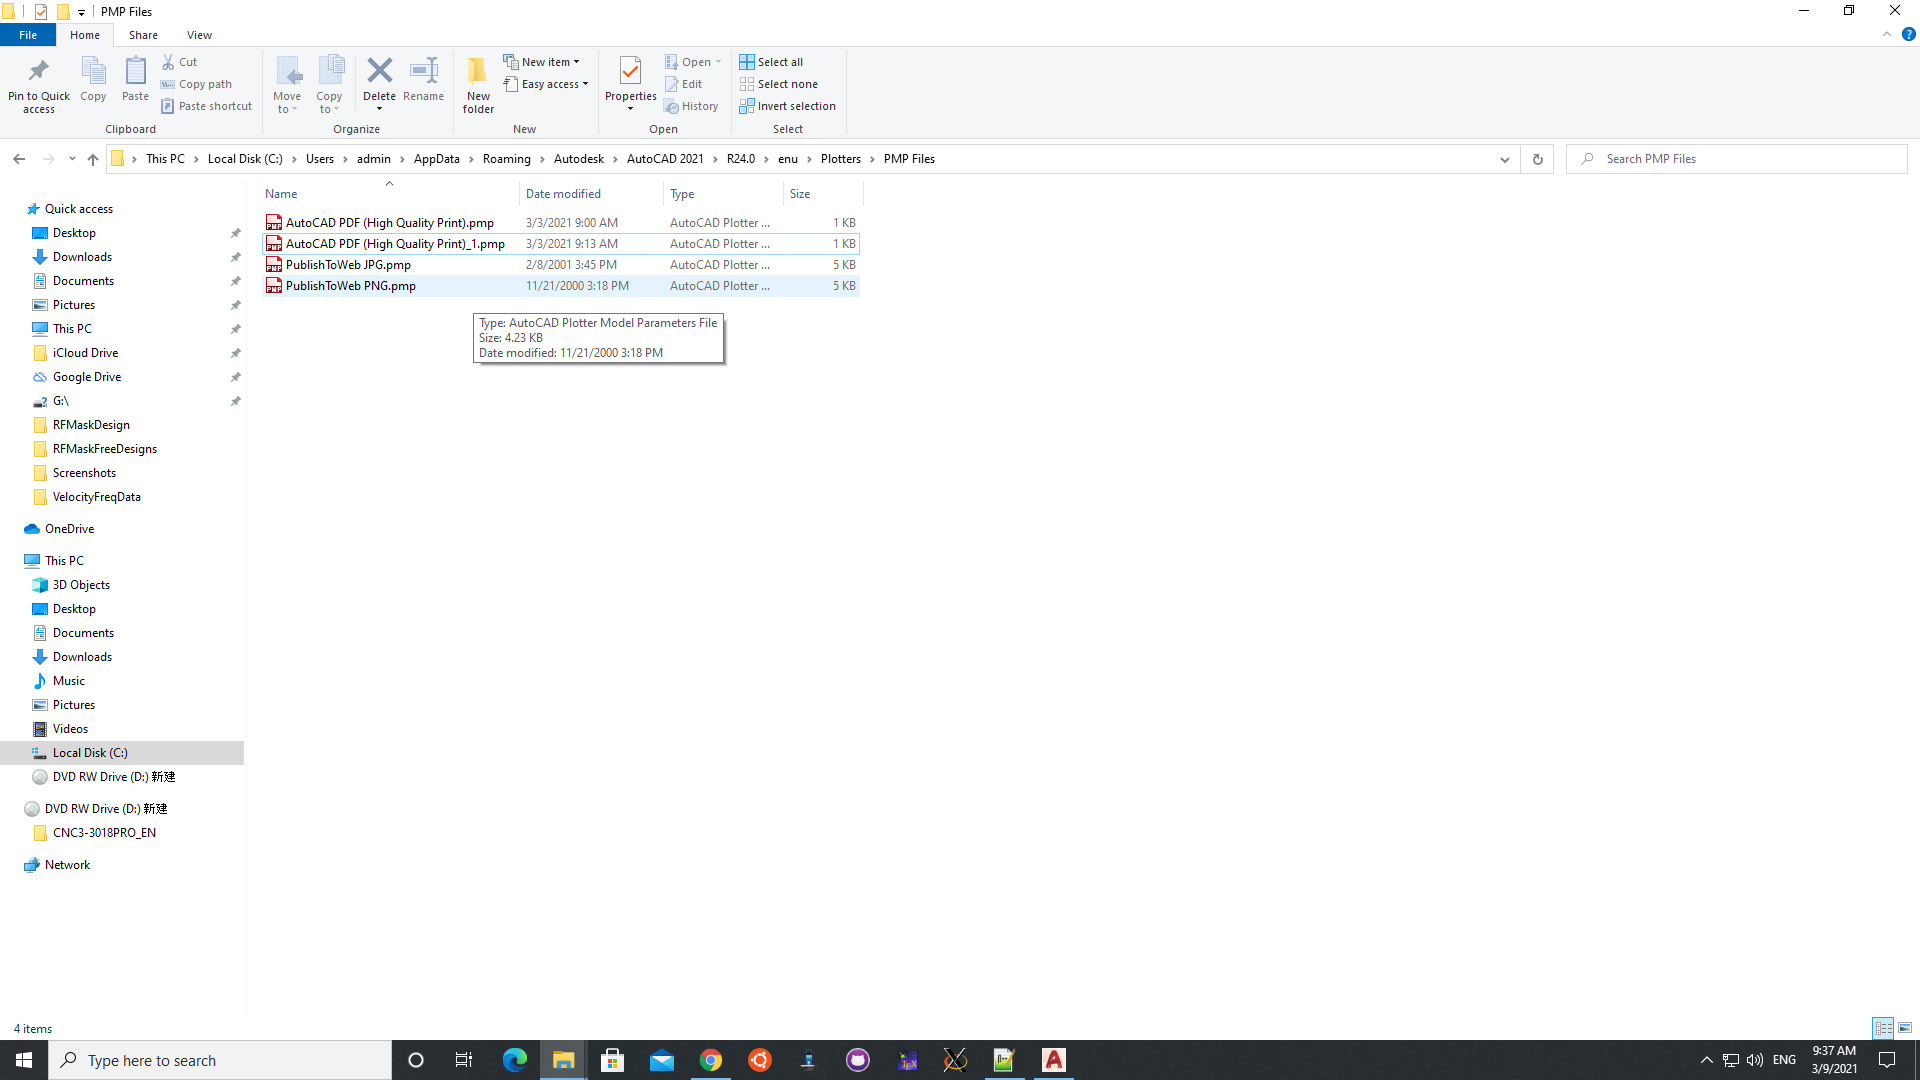
\includegraphics[angle=0,origin=c,width = .8\linewidth]{Section_ODMR_Antenna/Figures/FolderOfCustomPlotters.png}
		\caption{Customized plotter file in AutoCAD Plotters folder.}
		\label{fig:FolderOfCustomPlotters}
	\end{figure}

	\item Click on "OK" in "Plotter Configuration Editor" window to close it.

	\item In "Plot - Model" window, under "Plot Area" section, change "What to Plot:" to "Extents",
	Figure\ref{fig:DefinePlotArea}.
	
	\begin{figure}[H]
		\centering
		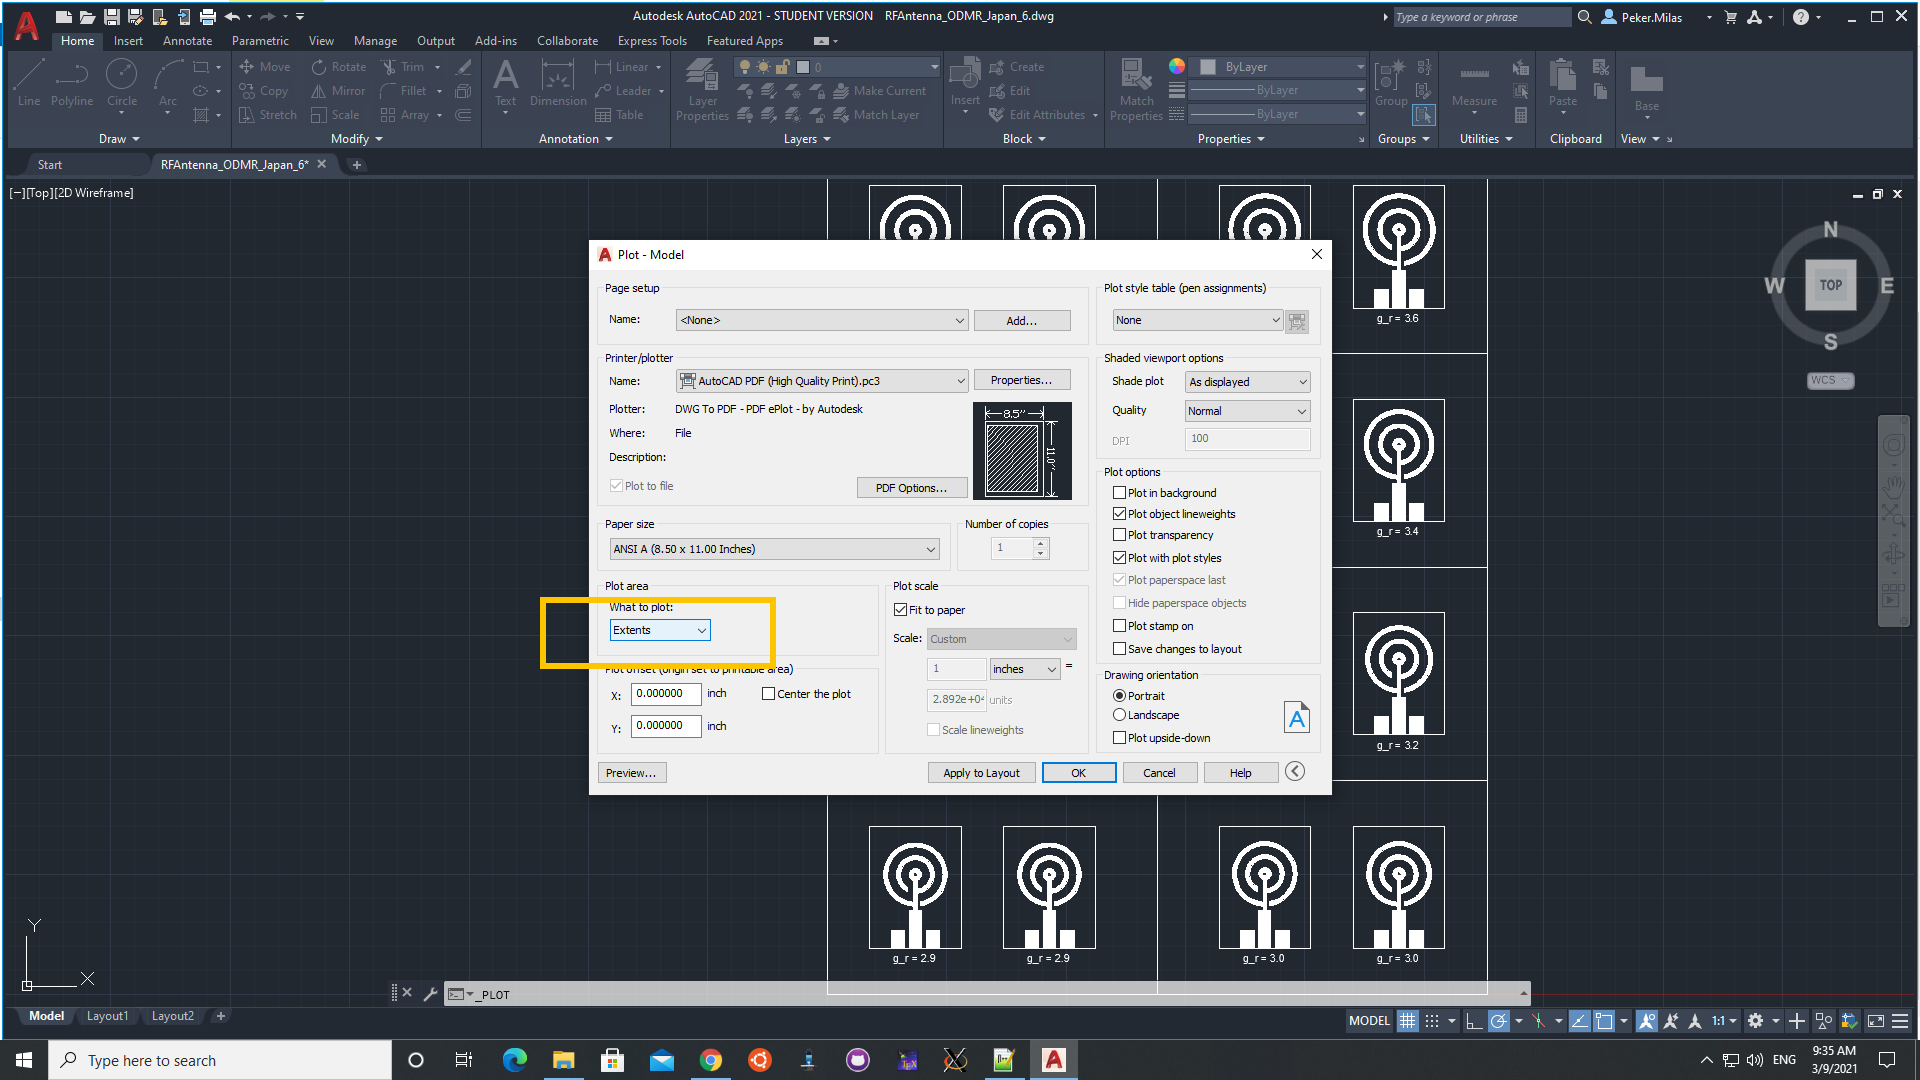
\includegraphics[angle=0,origin=c,width = .8\linewidth]{Section_ODMR_Antenna/Figures/DefinePlotArea.png}
		\caption{Selection of plot area in "Plot - Model" window.}
		\label{fig:DefinePlotArea}
	\end{figure}
	
	\item In "Plot - Model" window, under "Shaded vieport options" section, change "Quality" to "Maximum",
	Figure\ref{fig:PrintQuality}.

	\begin{figure}[H]
		\centering
		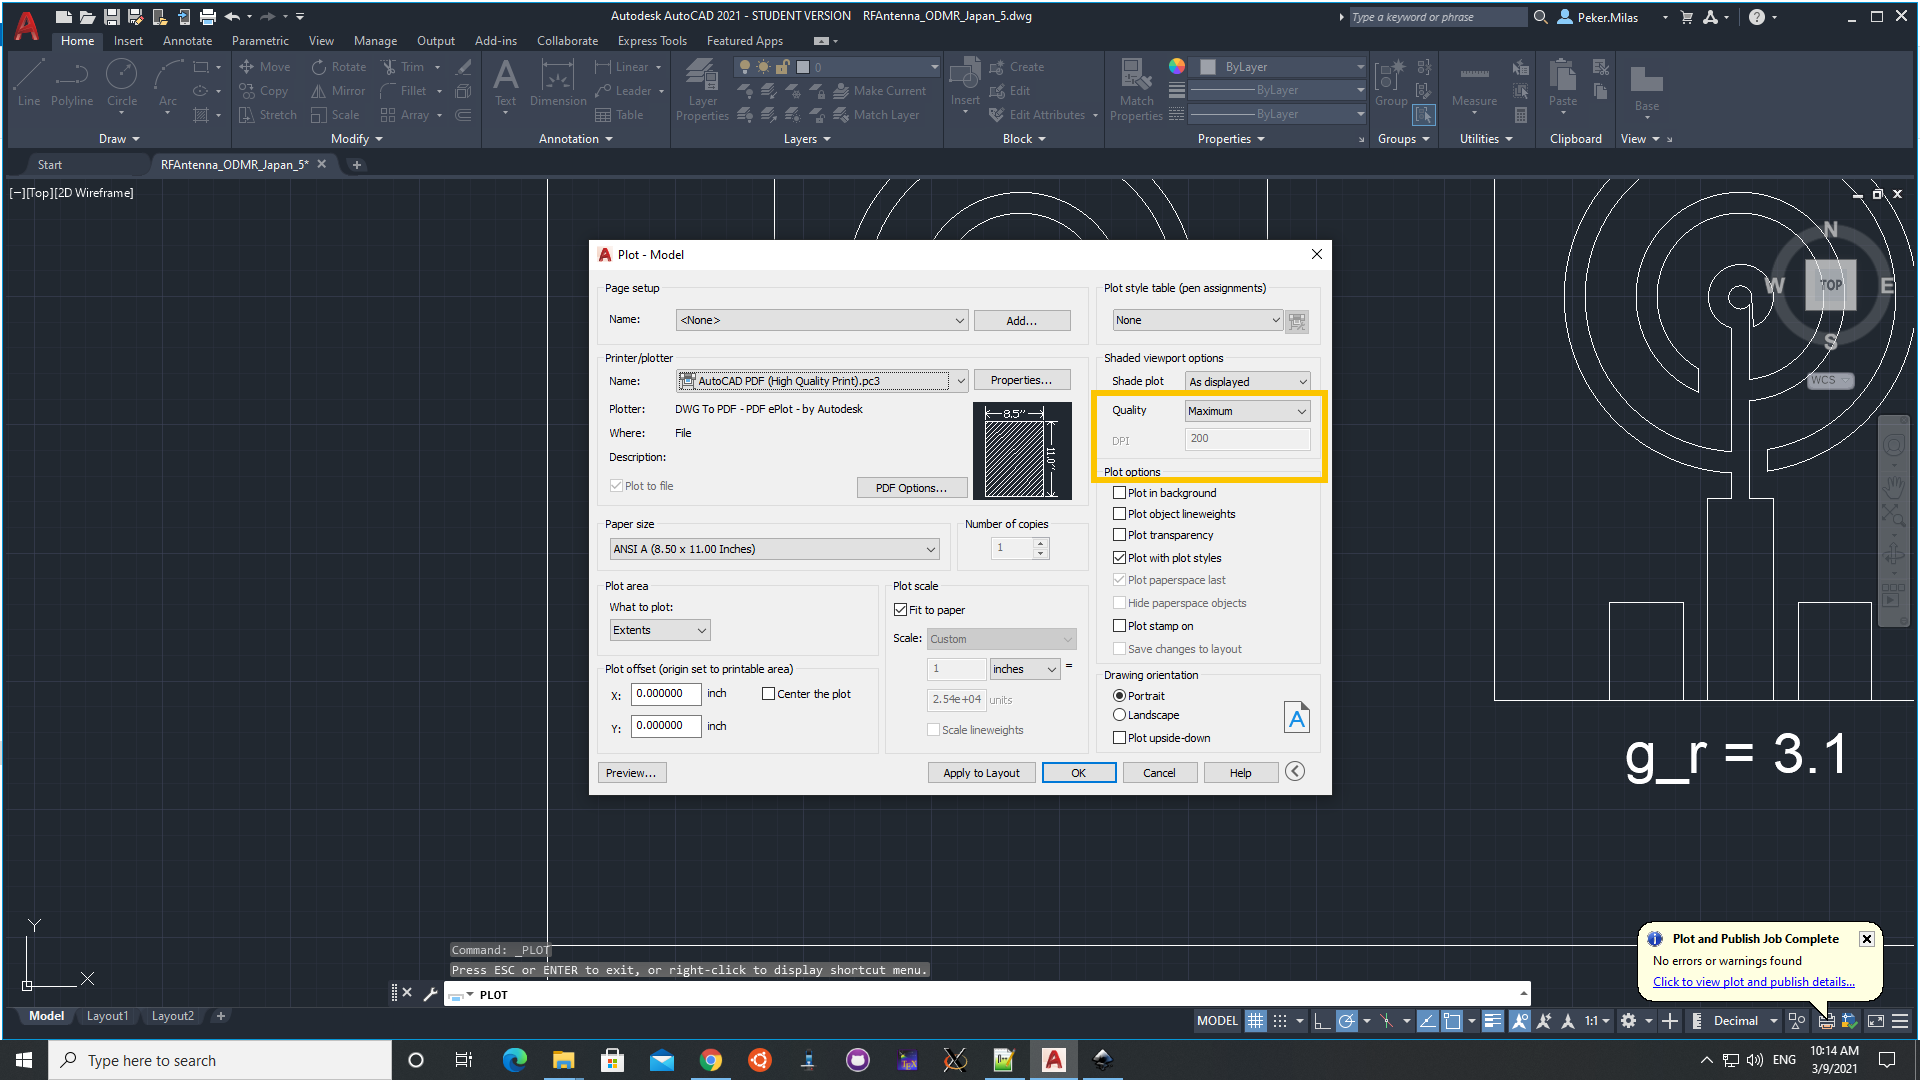
\includegraphics[angle=0,origin=c,width = .8\linewidth]{Section_ODMR_Antenna/Figures/PrintQuality.png}
		\caption{Setting plot quality in "Plot - Model" window.}
		\label{fig:PrintQuality}
	\end{figure}
	
	\item In "Plot - Model" window, under "Plot options" section, un-click "Plot object lineweights" box,
	Figure\ref{fig:PrintLineweights}.
	
	\begin{figure}[H]
		\centering
		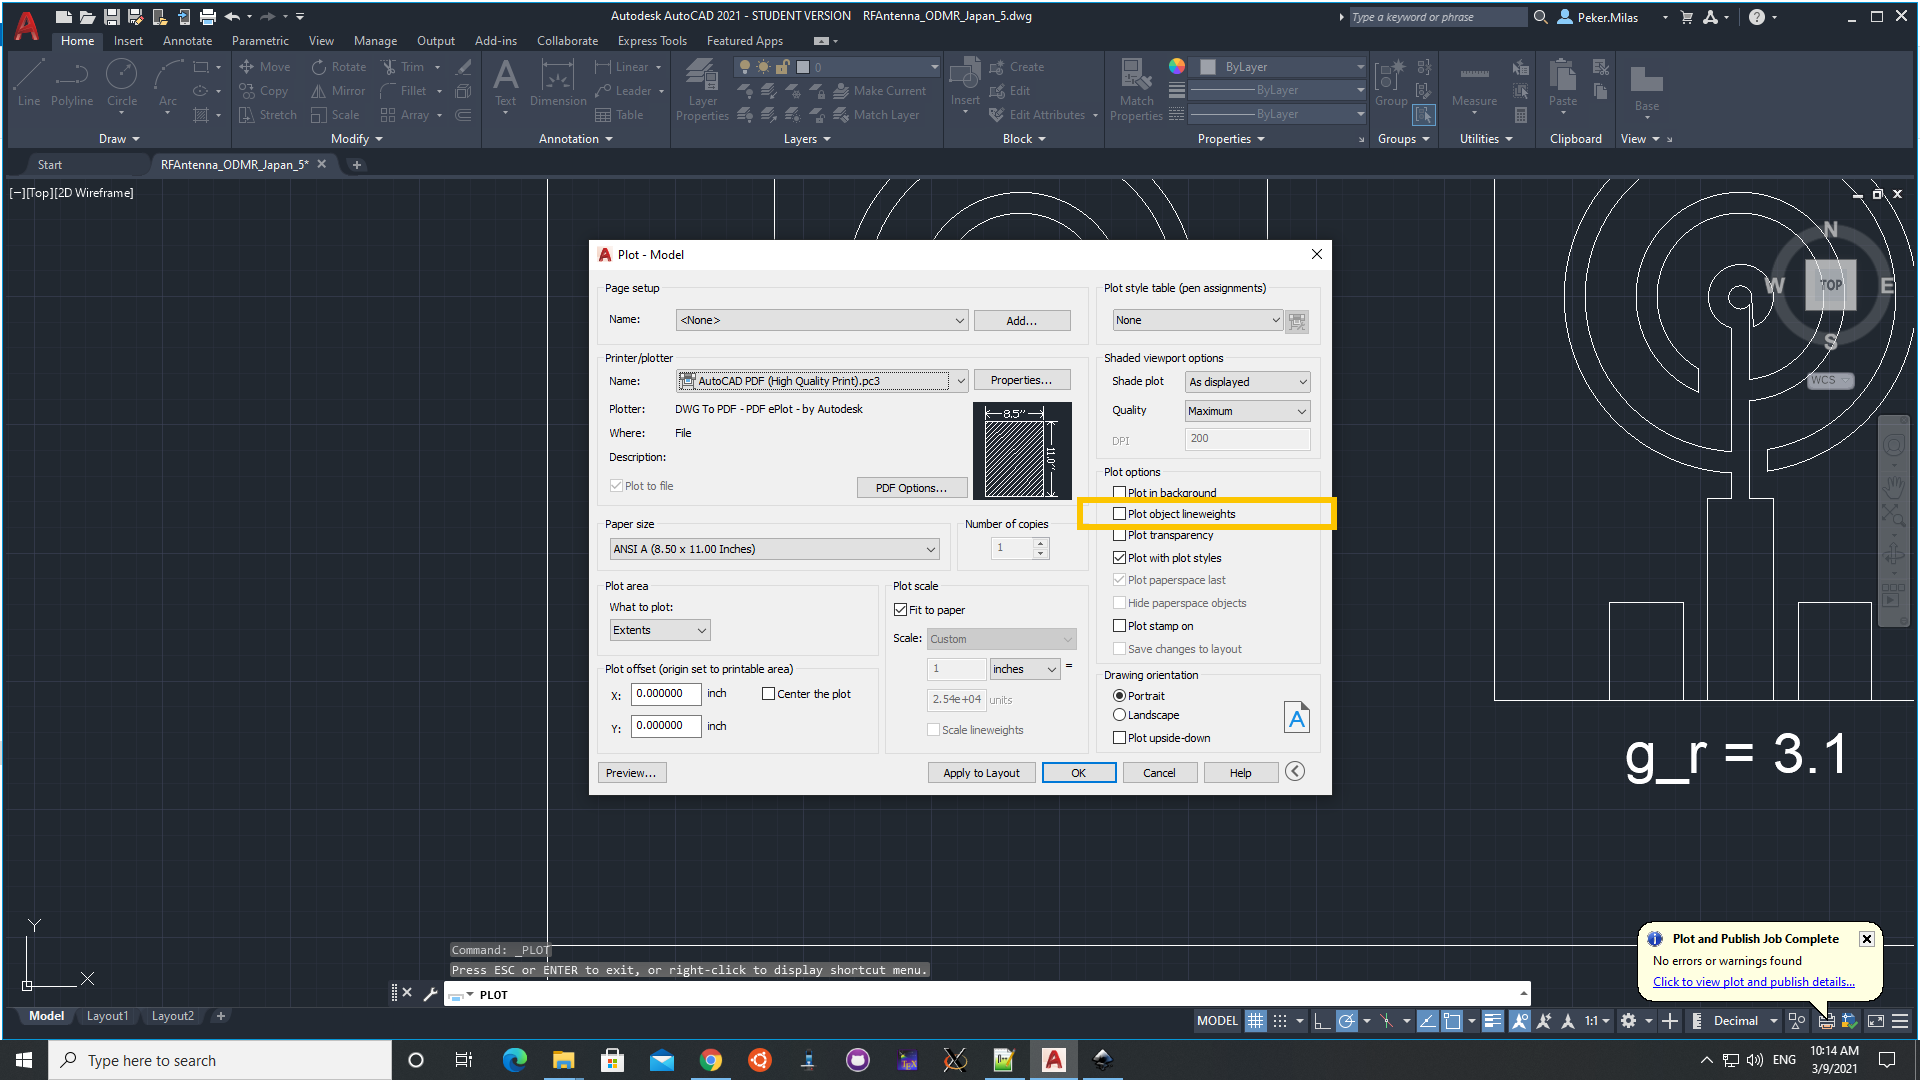
\includegraphics[angle=0,origin=c,width = .8\linewidth]{Section_ODMR_Antenna/Figures/PrintLineweights.png}
		\caption{Setting the plot line thicknesses to zero in "Plot - Model" window.}
		\label{fig:PrintLineweights}
	\end{figure}

	\item Now the drawing can be plotted/converted to a .pdf file.
	
\end{enumerate}

Following the conversion of the drawing, the resultant .pdf file needs to be post-processed with Inkscape.
This has to be done in following steps;

\begin{enumerate}
	
	\item Open the .pdf file in Inkscape. In "Import" window select Poppler/Cairo option,
	Figure\ref{fig:OpenPdfInkscape}.
	
	\begin{figure}[H]
		\centering
		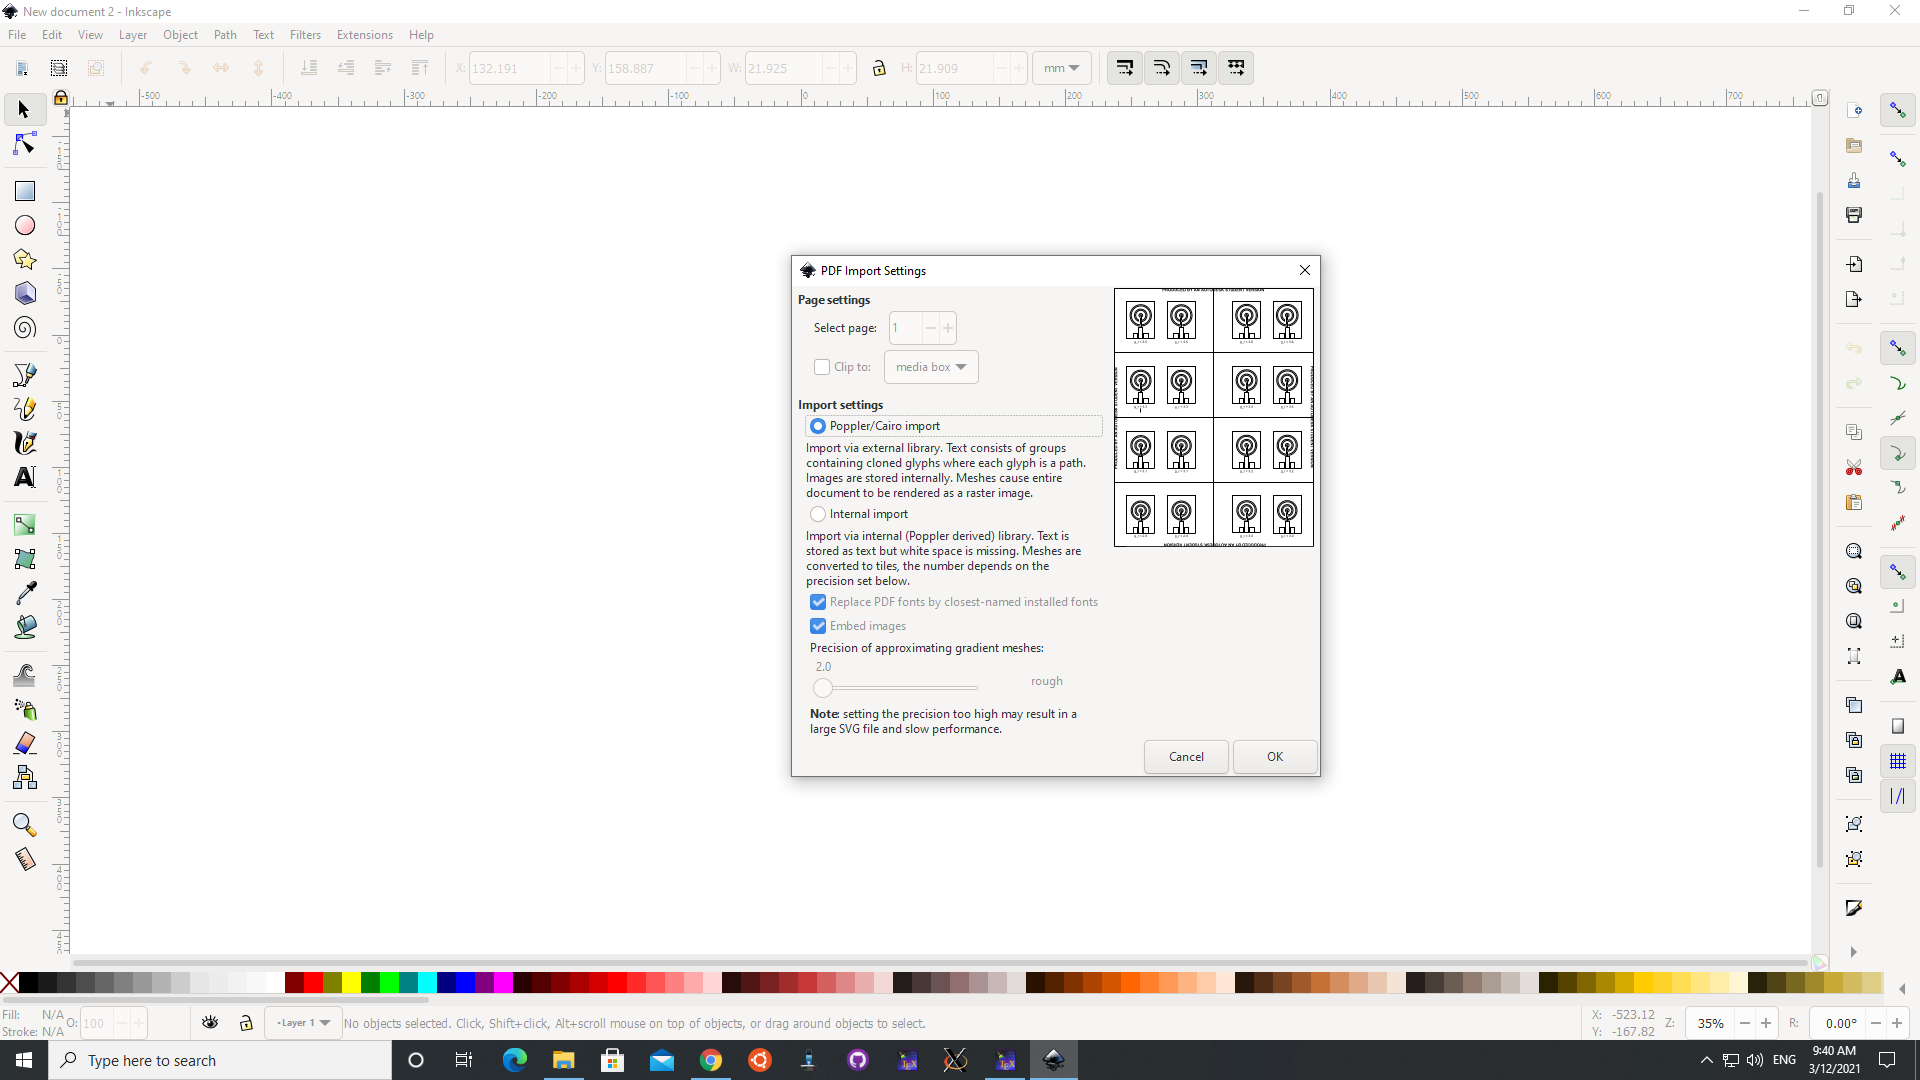
\includegraphics[angle=0,origin=c,width = .8\linewidth]{Section_ODMR_Antenna/Figures/OpenPdfInkscape.png}
		\caption{Opening/Importing pdf version of the mask in Inkscape.}
		\label{fig:OpenPdfInkscape}
	\end{figure}
	
	
	\item Select everything and un-group, Figure\ref{fig:SelectUngroup}.

	\begin{figure}[H]
		\centering
		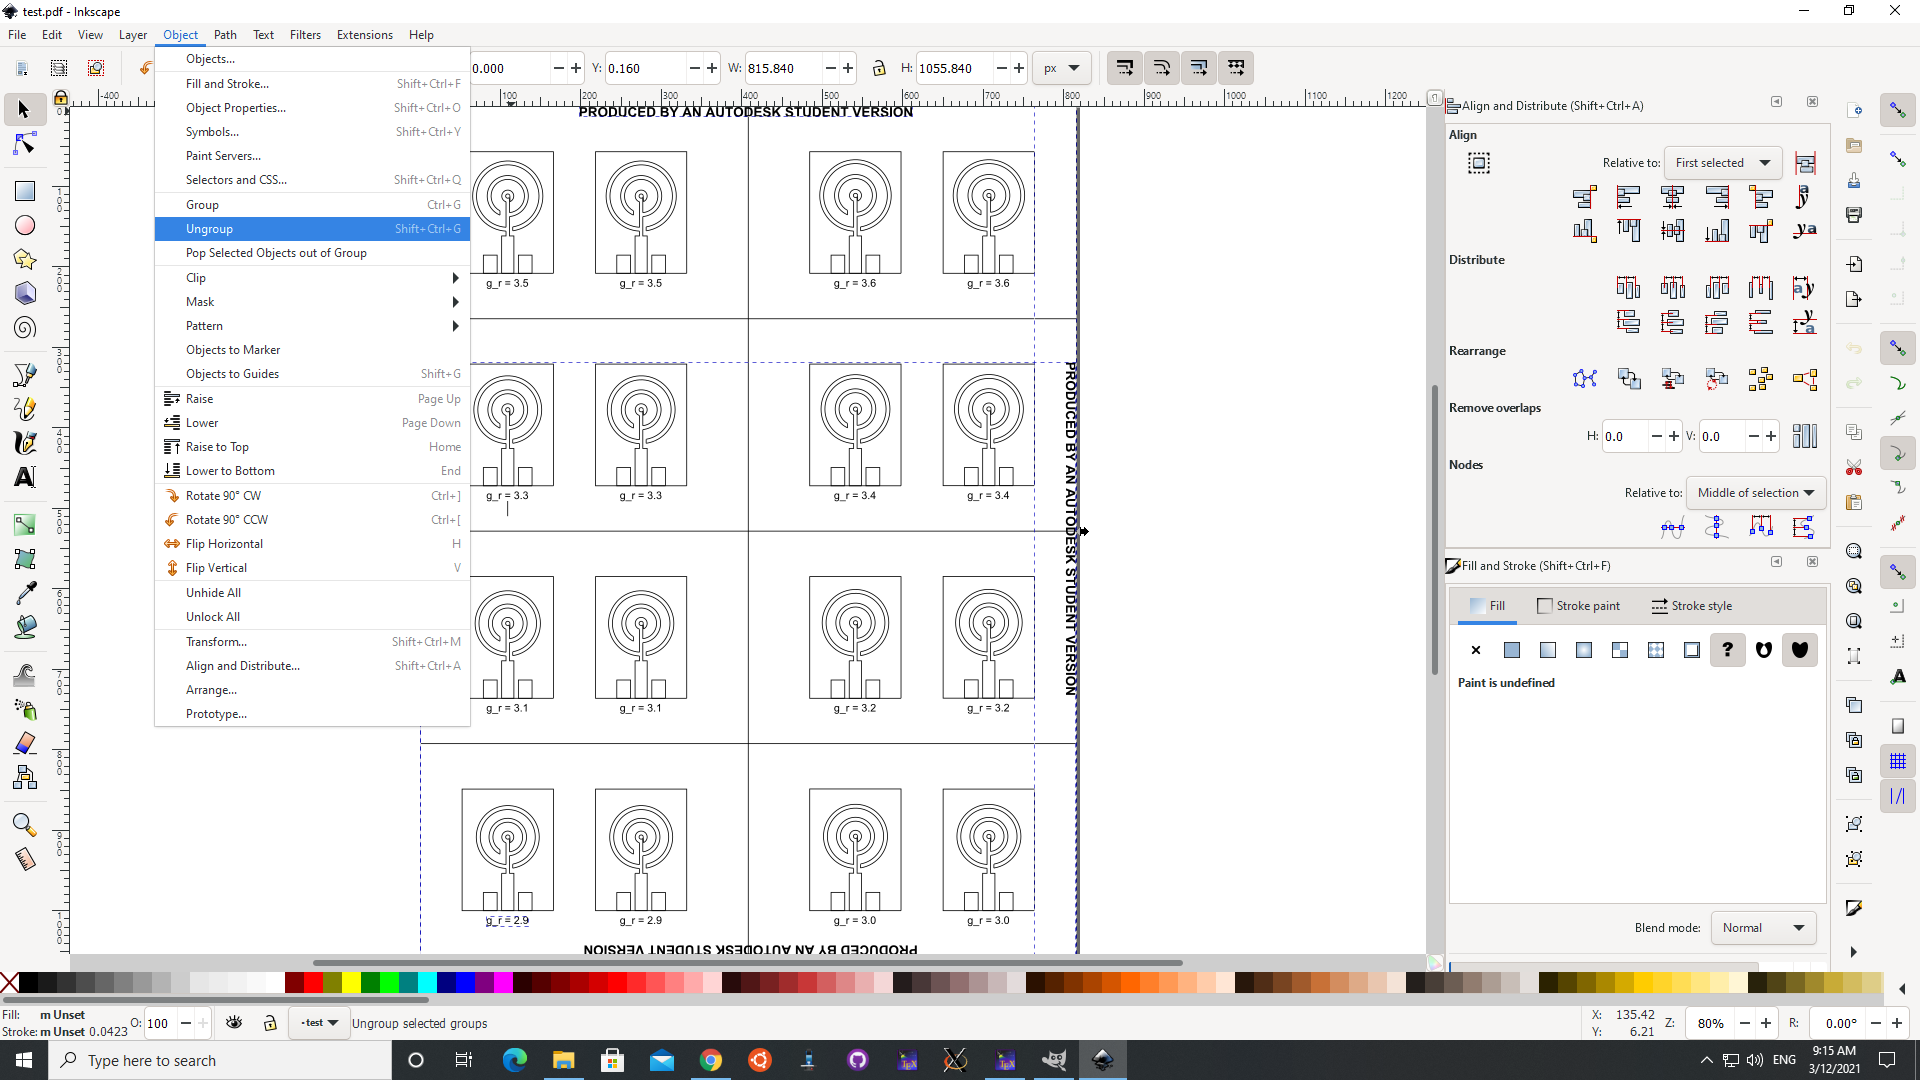
\includegraphics[angle=0,origin=c,width = .8\linewidth]{Section_ODMR_Antenna/Figures/SelectUngroup.png}
		\caption{Ungrouping the selected elements in Inkscape.}
		\label{fig:SelectUngroup}
	\end{figure}
	
	\item Click on "Edit nodes" and select disconnected line segments. Selection of disconnected 
	line segments can be done by left-clicking on a line segment while holding "Shift" button, 
	Figure\ref{fig:EditNodes}.
	
	\begin{figure}[H]
		\centering
		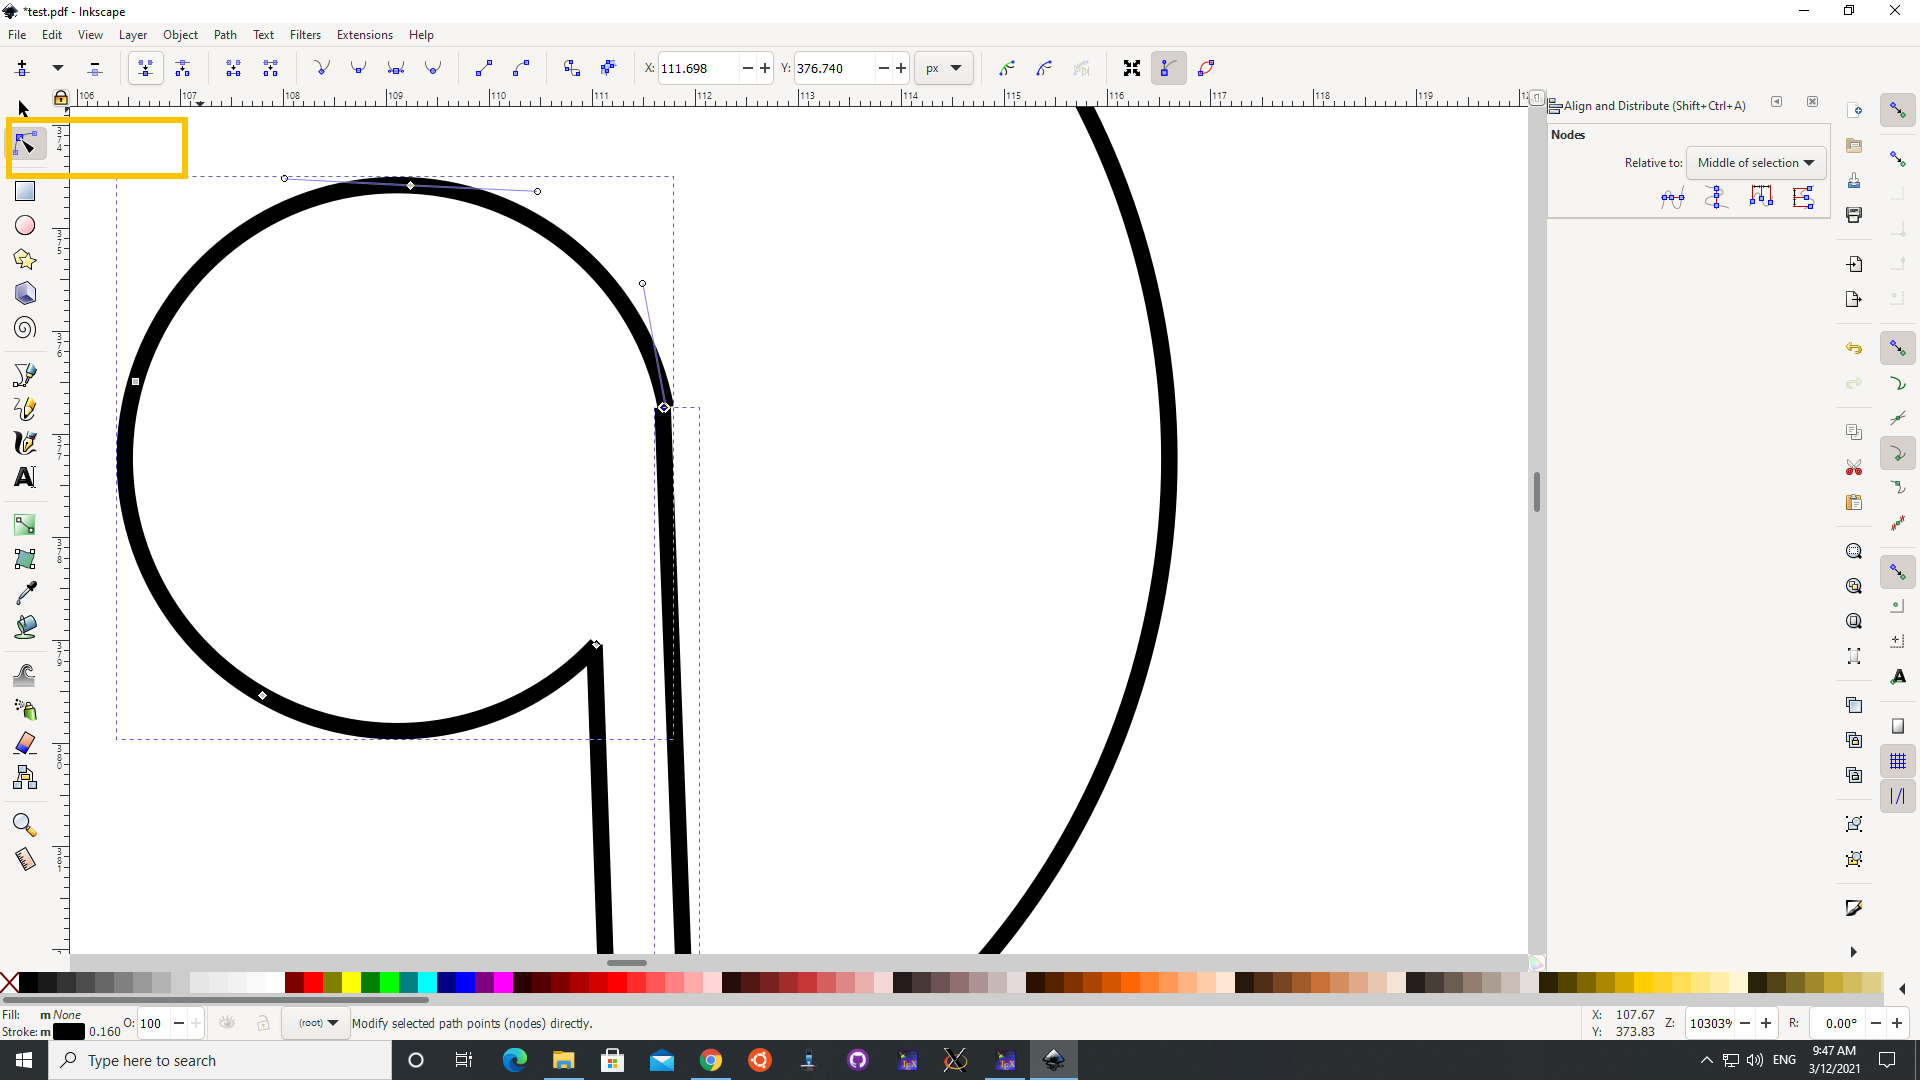
\includegraphics[angle=0,origin=c,width = .8\linewidth]{Section_ODMR_Antenna/Figures/EditNodes.png}
		\caption{Selection of Edit Nodes and the two disconnected line segments in Inkscape.}
		\label{fig:EditNodes}
	\end{figure}

	\item By looking at the zoomed in images, disconnected line segments' ends will be obvious.
	Here select these line segment ends and "Join" them. This has to be done for all disconnected
	line segments, Figure\ref{fig:JoinNodes}.

	\begin{figure}[H]
		\centering
		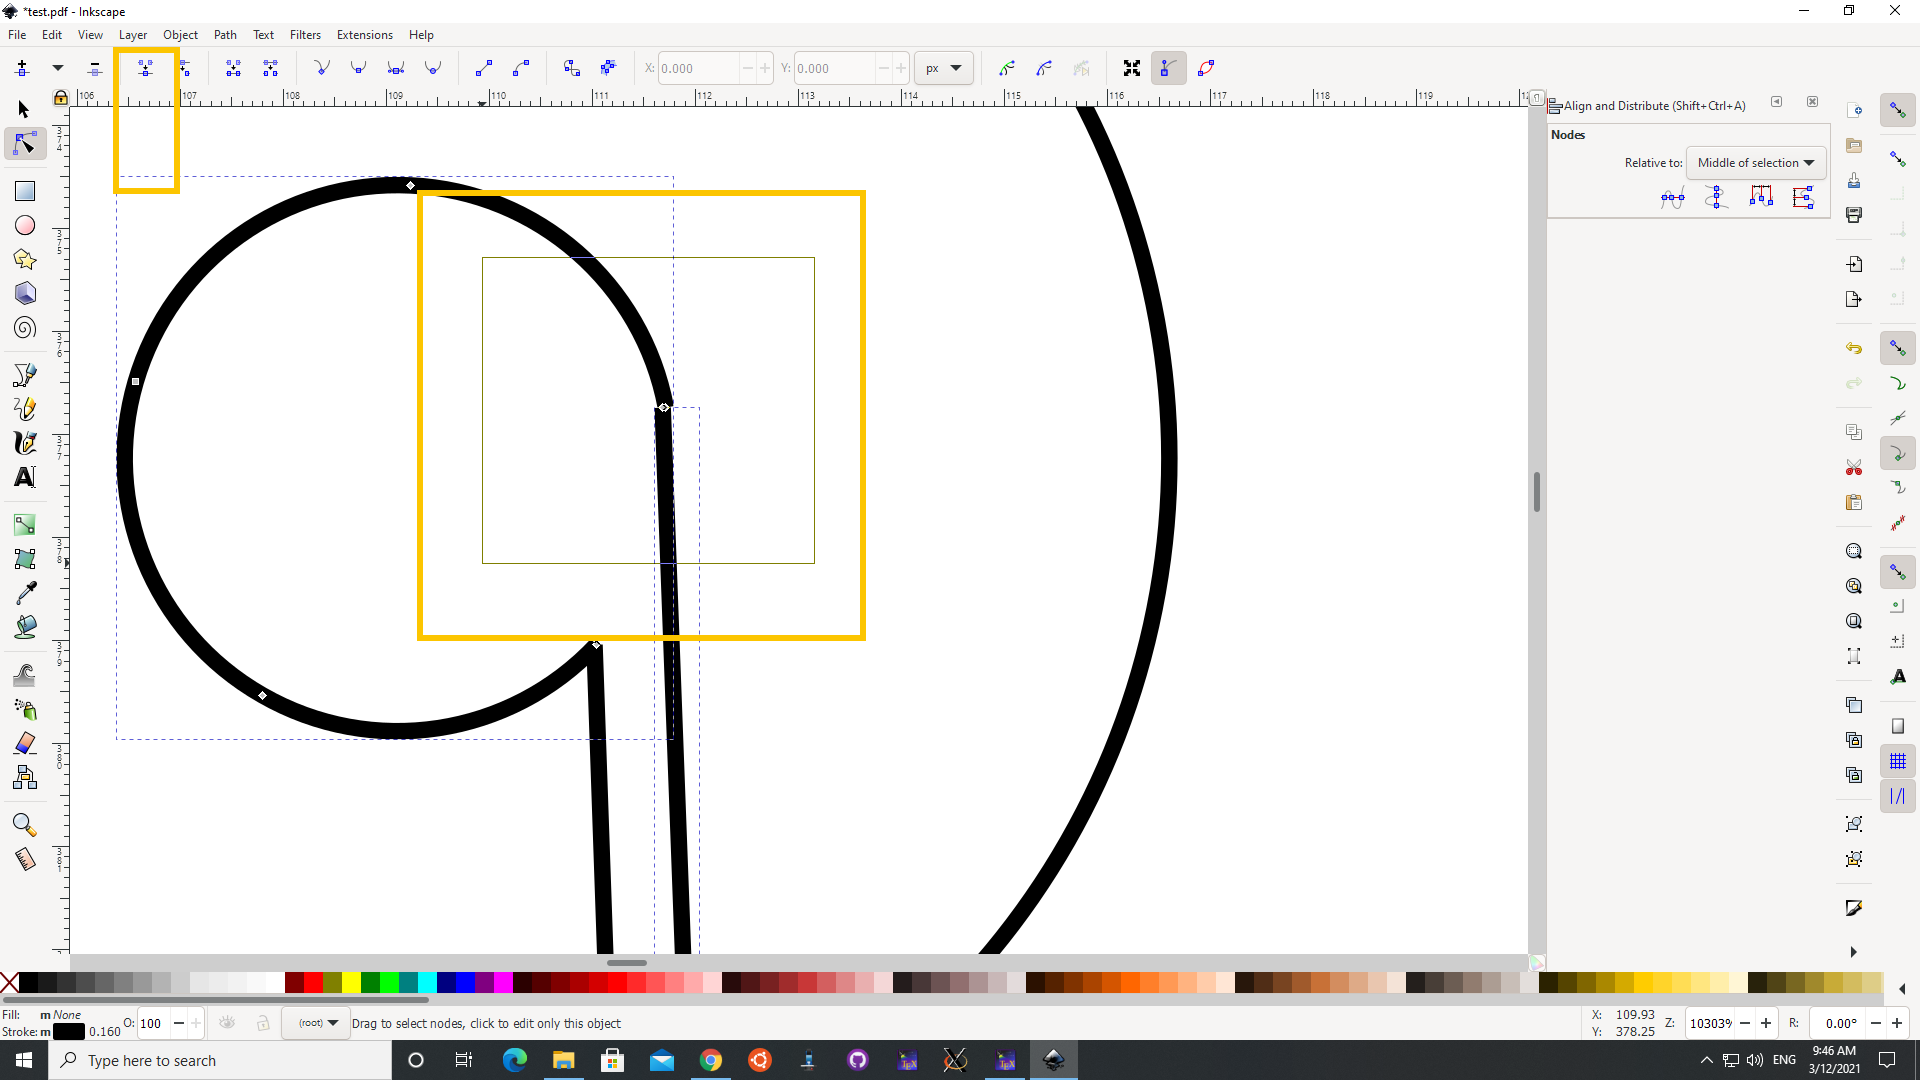
\includegraphics[angle=0,origin=c,width = .8\linewidth]{Section_ODMR_Antenna/Figures/JoinNodes.png}
		\caption{Joining the end nodes of two disconnected line segments in Inkscape.}
		\label{fig:JoinNodes}
	\end{figure}
	
	\item Processing fully connected structures is very easy in Inkscape, so additional changes in
	the document without disturbing the original design can be done at this stage. One example to
	these changes can be increasing the number of structures or repositioning them with respect to
	the page.
	
	\item Select the fully connected structure and open up "Fill and Stroke" dialog, Figure\ref{fig:FillAndStroke}. 

	\begin{figure}[H]
		\centering
		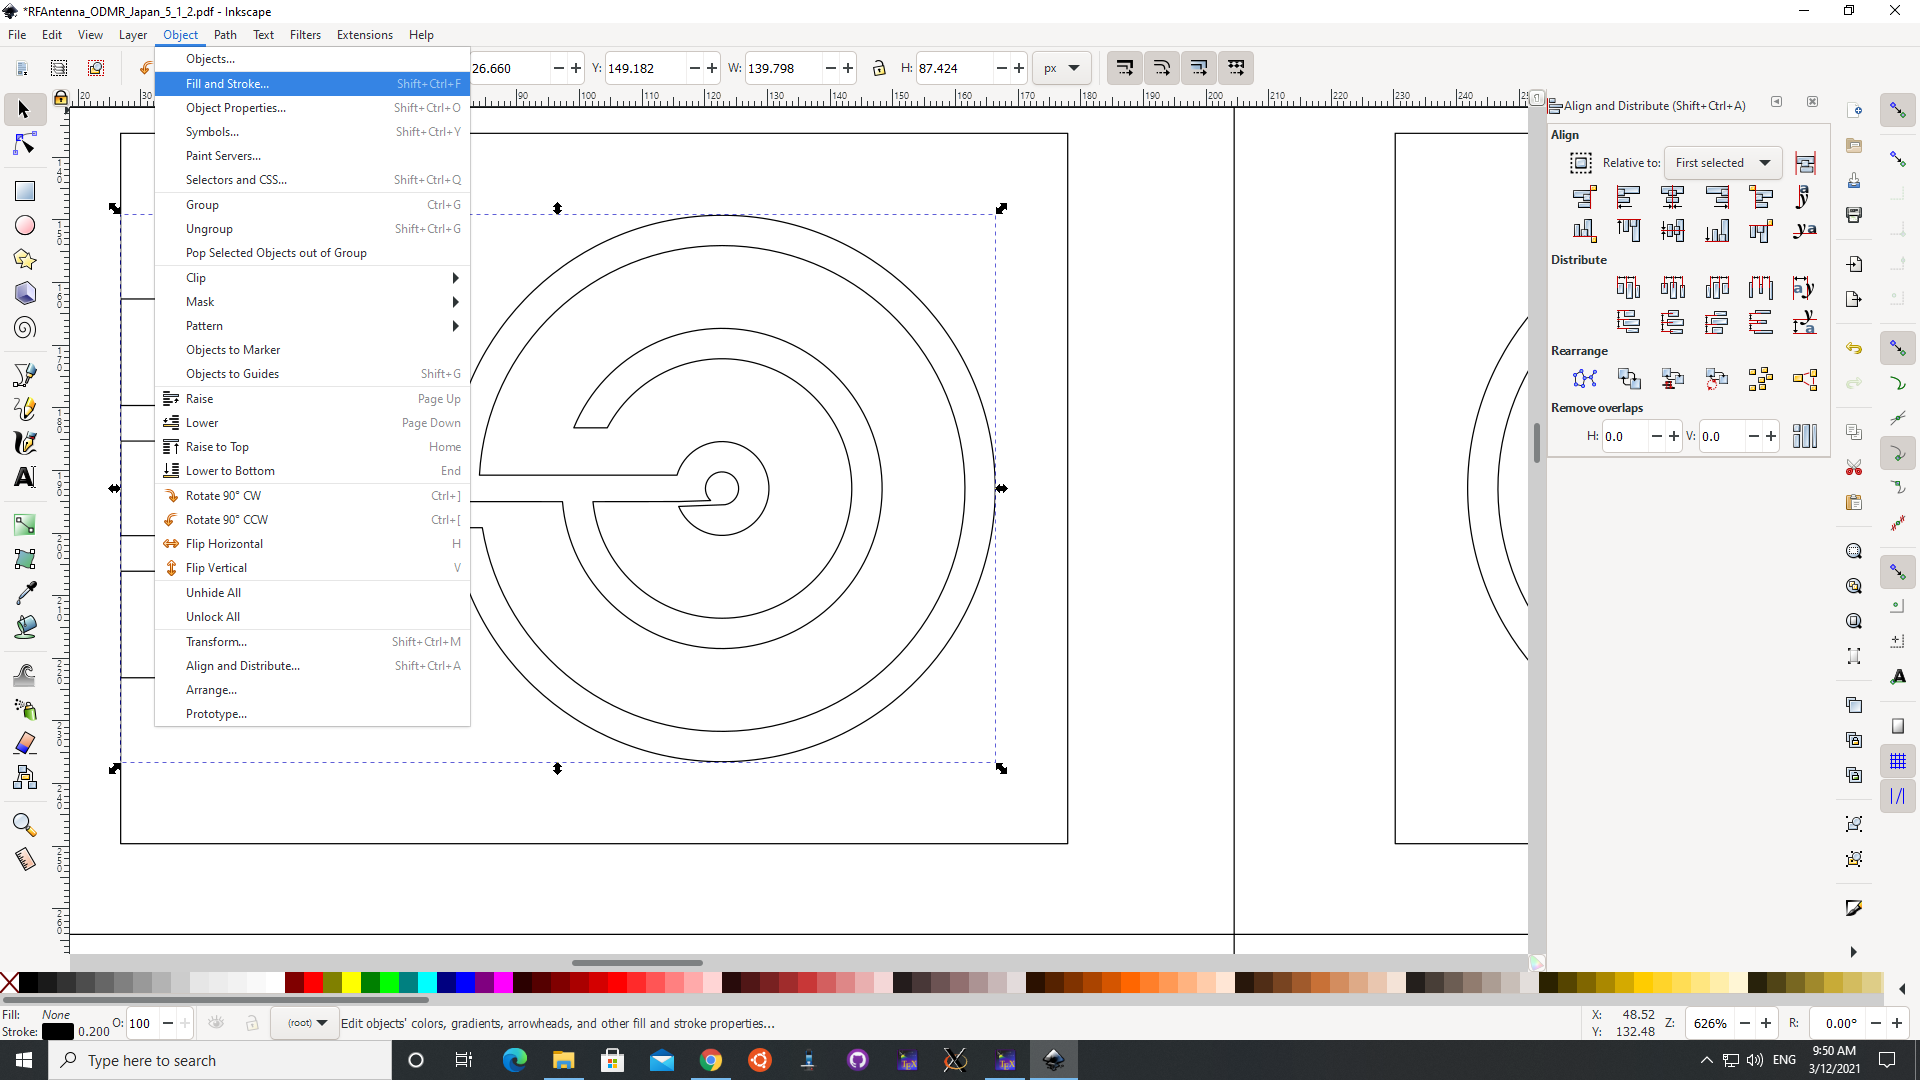
\includegraphics[angle=0,origin=c,width = .8\linewidth]{Section_ODMR_Antenna/Figures/FillAndStroke.png}
		\caption{Fill and Stroke dialog in Inkscape.}
		\label{fig:FillAndStroke}
	\end{figure}
	
	\item In "Fill and Stroke" dialog, Fill with a solid color, Figure\ref{fig:FillSolidColor}. 

	\begin{figure}[H]
		\centering
		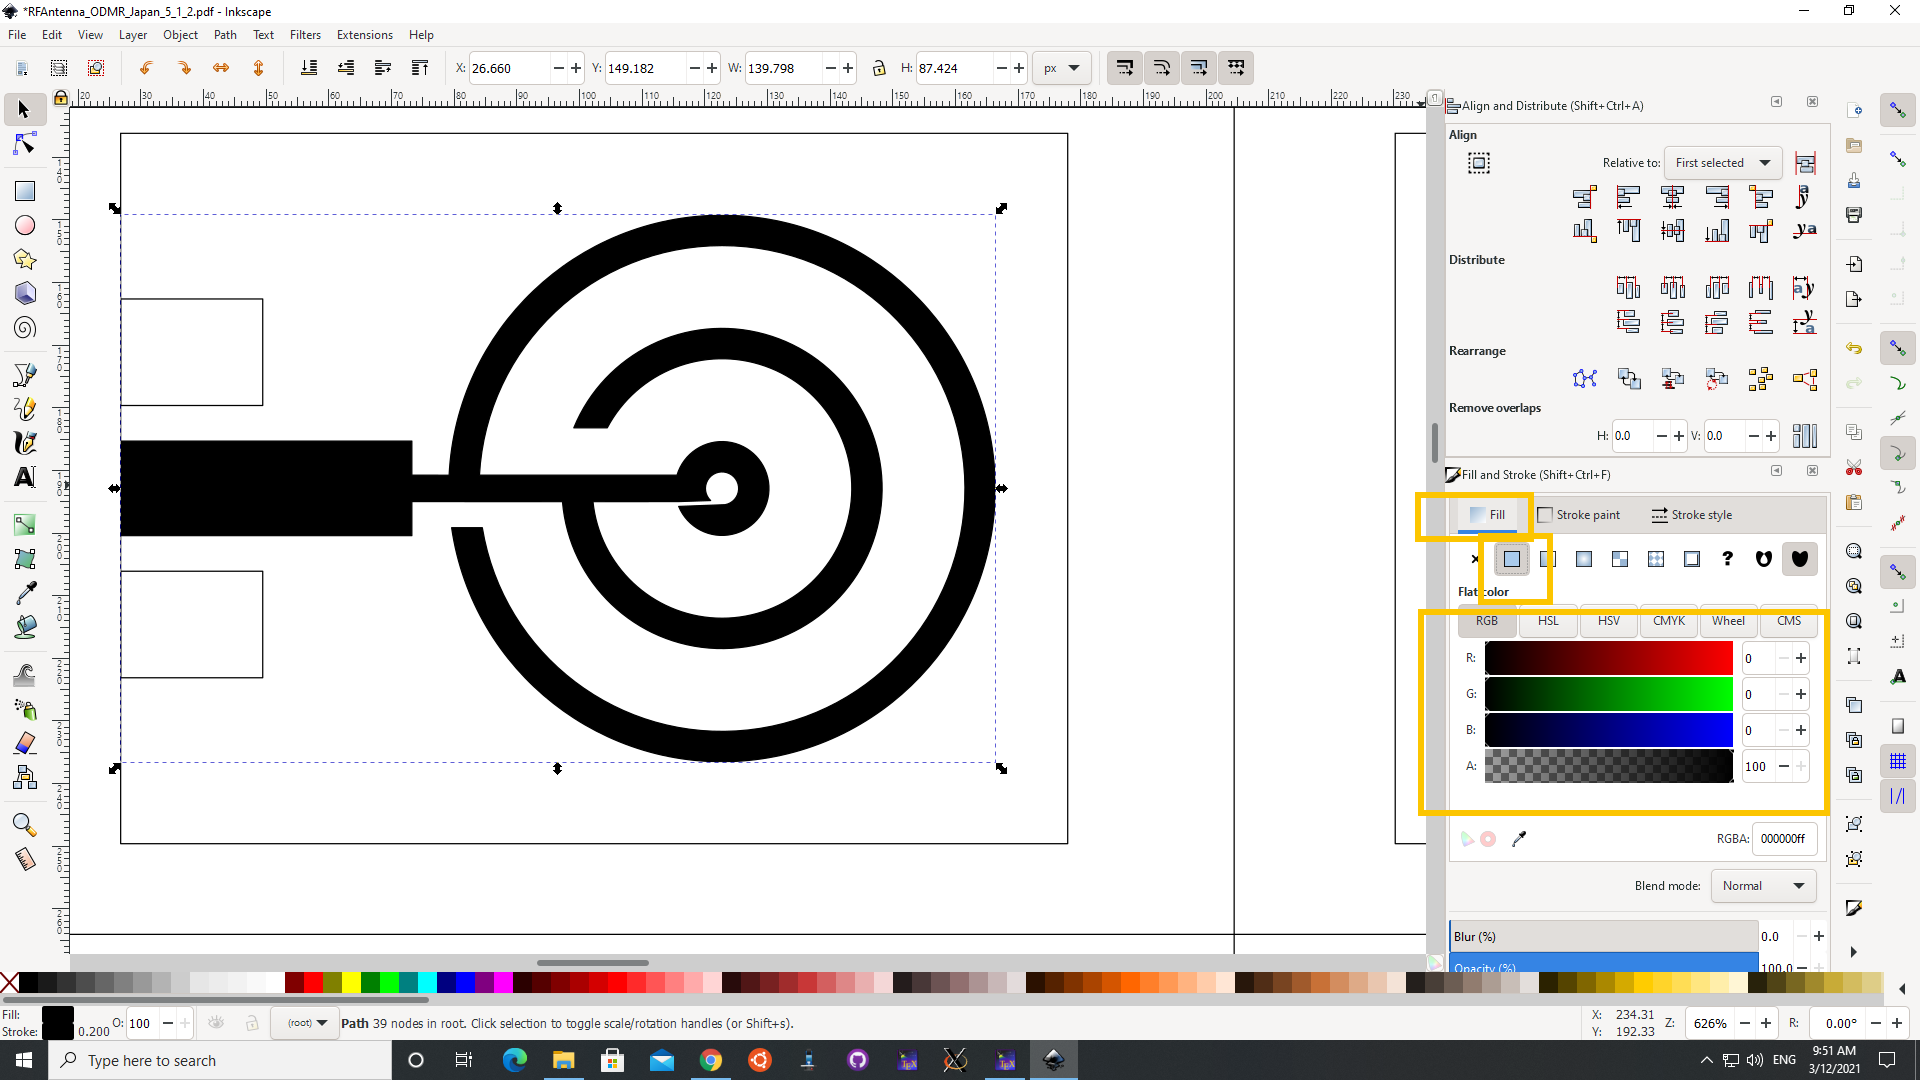
\includegraphics[angle=0,origin=c,width = .8\linewidth]{Section_ODMR_Antenna/Figures/FillSolidColor.png}
		\caption{Filling structures with a solid color in Inkscape.}
		\label{fig:FillSolidColor}
	\end{figure}
	
	\item Select everything on the page and group them this time from the menu that was used for
	un-grouping, Figure\ref{fig:SelectUngroup}.
	
	\item Save the final design as \textbf{.svg} file first. Then save it again as \textbf{.pdf} file.
\end{enumerate}



\subsubsection{Lithography on Copper Laminate}

AAA
